%%%%%%%%%%%%%%%%%%%%%%%%%%%%%%%%%%%%%%%%%
% Journal Article
% LaTeX Template
% Version 1.3 (9/9/13)
%
% This template has been downloaded from:
% http://www.LaTeXTemplates.com
%
% Original author:
% Frits Wenneker (http://www.howtotex.com)
%
% License:
% CC BY-NC-SA 3.0 (http://creativecommons.org/licenses/by-nc-sa/3.0/)
%
%%%%%%%%%%%%%%%%%%%%%%%%%%%%%%%%%%%%%%%%%

%----------------------------------------------------------------------------------------
%  PACKAGES AND OTHER DOCUMENT CONFIGURATIONS
%----------------------------------------------------------------------------------------

\documentclass[twoside]{article}\usepackage[]{graphicx}\usepackage[]{color}
%% maxwidth is the original width if it is less than linewidth
%% otherwise use linewidth (to make sure the graphics do not exceed the margin)
\makeatletter
\def\maxwidth{ %
  \ifdim\Gin@nat@width>\linewidth
    \linewidth
  \else
    \Gin@nat@width
  \fi
}
\makeatother

\definecolor{fgcolor}{rgb}{0.345, 0.345, 0.345}
\newcommand{\hlnum}[1]{\textcolor[rgb]{0.686,0.059,0.569}{#1}}%
\newcommand{\hlstr}[1]{\textcolor[rgb]{0.192,0.494,0.8}{#1}}%
\newcommand{\hlcom}[1]{\textcolor[rgb]{0.678,0.584,0.686}{\textit{#1}}}%
\newcommand{\hlopt}[1]{\textcolor[rgb]{0,0,0}{#1}}%
\newcommand{\hlstd}[1]{\textcolor[rgb]{0.345,0.345,0.345}{#1}}%
\newcommand{\hlkwa}[1]{\textcolor[rgb]{0.161,0.373,0.58}{\textbf{#1}}}%
\newcommand{\hlkwb}[1]{\textcolor[rgb]{0.69,0.353,0.396}{#1}}%
\newcommand{\hlkwc}[1]{\textcolor[rgb]{0.333,0.667,0.333}{#1}}%
\newcommand{\hlkwd}[1]{\textcolor[rgb]{0.737,0.353,0.396}{\textbf{#1}}}%

\usepackage{framed}
\makeatletter
\newenvironment{kframe}{%
 \def\at@end@of@kframe{}%
 \ifinner\ifhmode%
  \def\at@end@of@kframe{\end{minipage}}%
  \begin{minipage}{\columnwidth}%
 \fi\fi%
 \def\FrameCommand##1{\hskip\@totalleftmargin \hskip-\fboxsep
 \colorbox{shadecolor}{##1}\hskip-\fboxsep
     % There is no \\@totalrightmargin, so:
     \hskip-\linewidth \hskip-\@totalleftmargin \hskip\columnwidth}%
 \MakeFramed {\advance\hsize-\width
   \@totalleftmargin\z@ \linewidth\hsize
   \@setminipage}}%
 {\par\unskip\endMakeFramed%
 \at@end@of@kframe}
\makeatother

\definecolor{shadecolor}{rgb}{.97, .97, .97}
\definecolor{messagecolor}{rgb}{0, 0, 0}
\definecolor{warningcolor}{rgb}{1, 0, 1}
\definecolor{errorcolor}{rgb}{1, 0, 0}
\newenvironment{knitrout}{}{} % an empty environment to be redefined in TeX

\usepackage{alltt}

\usepackage{lipsum} % Package to generate dummy text throughout this template

\usepackage[sc]{mathpazo} % Use the Palatino font
%\usepackage[T1]{fontenc} % Use 8-bit encoding that has 256 glyphs
\usepackage[utf8]{inputenc}
\linespread{1.05} % Line spacing - Palatino needs more space between lines
\usepackage{microtype} % Slightly tweak font spacing for aesthetics

\usepackage[hmarginratio=1:1,top=32mm,columnsep=20pt]{geometry} % Document margins
\usepackage{multicol} % Used for the two-column layout of the document
\usepackage{float} %we need this to use figure environments within multicol. knitr figure chunks need to include fig.pos='H'. 'H' stems from package float and deactivates floating (which multicol does not like)
\usepackage[hang, small,labelfont=bf,up,textfont=it,up]{caption} % Custom captions under/above floats in tables or figures
\usepackage{booktabs} % Horizontal rules in tables
\usepackage{float} % Required for tables and figures in the multi-column environment - they need to be placed in specific locations with the [H] (e.g. \begin{table}[H])
\usepackage{hyperref} % For hyperlinks in the PDF
\usepackage{graphicx}
\usepackage{datetime} %for automatic date in the header

\usepackage{lettrine} % The lettrine is the first enlarged letter at the beginning of the text
\usepackage{paralist} % Used for the compactitem environment which makes bullet points with less space between them

\usepackage{color} % used to mark parts that need to be edited
\usepackage[comma,authoryear]{natbib} %to use citealt citet citep
%\usepackage{biblatex} %to make use of the date field in .bib-files instead of year-field.
%\usepackage{url}
\usepackage{abstract} % Allows abstract customization
\renewcommand{\abstractnamefont}{\normalfont\bfseries} % Set the "Abstract" text to bold
\renewcommand{\abstracttextfont}{\normalfont\small\itshape} % Set the abstract itself to small italic text

%%%%%% new command to break multicol environment from time to time
\newcounter{tempcolnum}
\makeatletter
\newcommand{\multicolinterrupt}[1]{% Stuff to span both rows
\setcounter{tempcolnum}{\col@number}
\end{multicols}
#1%
\begin{multicols}{\value{tempcolnum}}
}
\makeatother
%%%%%%%

\usepackage{titlesec} % Allows customization of titles
\renewcommand\thesection{\Roman{section}} % Roman numerals for the sections
\renewcommand\thesubsection{\Roman{subsection}} % Roman numerals for subsections
\titleformat{\section}[block]{\large\scshape\centering}{\thesection.}{1em}{} % Change the look of the section titles
\titleformat{\subsection}[block]{\large}{\thesubsection.}{1em}{} % Change the look of the section titles

\usepackage{fancyhdr} % Headers and footers
\pagestyle{fancy} % All pages have headers and footers
\fancyhead{} % Blank out the default header
\fancyfoot{} % Blank out the default footer
\newdateformat{mydate}{\monthname[\THEMONTH] \THEYEAR}
\fancyhead[C]{Assessing income inequality with tax data $\bullet$ \mydate\today~$\bullet$ Working paper} % Custom header text
\fancyfoot[RO,LE]{\thepage} % Custom footer text
%\bibliographystyle{plain}
\bibliographystyle{unsrtnat}

%%%-------------------------------------------------%%%
%%% Preferences for Knitr %%%
%%%-------------------------------------------------%%%


%%%-------------------------------------------------%%%
%%% Sub document global preferences for Knitr %%%
%%%-------------------------------------------------%%%








%----------------------------------------------------------------------------------------
%  TITLE SECTION
%----------------------------------------------------------------------------------------

\title{\vspace{-15mm}\fontsize{24pt}{10pt}\selectfont\textbf{Assessing income inequality with tax data - Switzerland from 1917 to 2010}} % Article title

\author{
\large
\textsc{Oliver Hümbelin}\\[2mm] % Your name
\normalsize Bern University of Applied Sciences \\ % Your institution
\normalsize \href{mailto:oliver.huembelin@bfh.ch}{oliver.huembelin@bfh.ch} % Your email address
\vspace{5mm}\\
\large
\textsc{Rudolf Farys}\\[2mm] % Your name
\normalsize University of Bern \\ % Your institution
\normalsize \href{mailto:rudolf.farys@soz.unibe.ch}{rudolf.farys@soz.unibe.ch} % Your email address
\vspace{-5mm}
}
\date{}

%----------------------------------------------------------------------------------------
\IfFileExists{upquote.sty}{\usepackage{upquote}}{}
\begin{document}

\maketitle 

\thispagestyle{fancy} % All pages have headers and footers

%----------------------------------------------------------------------------------------
%	ABSTRACT
%----------------------------------------------------------------------------------------

%%%-------------------------------------------------%%%
%%% Include abstract %%%
%%%-------------------------------------------------%%%


%%%-------------------------------------------------%%%
%%% Sub document abstract %%%
%%%-------------------------------------------------%%%

\begin{abstract}
There is empirical evidence that economic inequality increased in the majority of western countries over the last decades (\citealt{oecd_divided_2011}, \citealt{gornick_income_2013}). 
In Switzerland, however, the development is unclear, as there is evidence for trends in both directions. Part of the inconclusive picture is due to different methodological approaches. In this paper we discuss the role of tax-data concerning the assessment of inequality in income. 
The focus of the discussion lays herein to show the benefits and shortcomings of tax data compared to current ``state of the art'' measurement concepts of economic inequality. 
We present common and new strategies to handle tax data specific methodological difficulties and compare results out of aggregated federal tax statistics to results from the Household Budget Survey (HBS). 
We find theoretical inconsistencies in both tax and survey data which both result in an underestimation of inequality.
Following the results from tax-data Switzerland experienced in slight rise in inequality in recent years, similar to other western countries due to a polarization of the income distribution.

% Salverda-Stuff und das neue Piketty Buch sollten irgendwo erwähnt werden



\end{abstract}


% Wir machen nichts mehr zu Vermögen (obwohl der Trend auch dahin geht, dass neben dem Einkommen auch das Vermögen eine zentrale Untersuchunsgrösse des inviduellen Wohlstandss darstellt)



%

% Alte version des abstractes. Fokus stärker auf Schweiz und Vermögen
%There is empirical evidence that economic inequality increased in the majority of western countries over the last decades (OECD, 2011; \citealt{gornick_income_2013}). In Switzerland, however, the development is unclear, as there is only little systematic evidence about income inequality that would allow for long-term comparison. Studies on the distribution of wealth are even scarcer. Nevertheless, income inequality has been a prominent theme in the public Swiss discussion in recent years, e.g. the most recent referendums "Abzockerinitiative'' and "1:12-Initiative''. We address the mentioned gap by presenting a long and consistent time series of inequality measures for income and wealth (1943-2010) calculated from federal tax statistics. We describe the benefits and shortcomings of tax data compared to other data sources and present strategies to handle tax data specific methodological difficulties. In the end we integrate the case of Switzerland into the international picture of inequality development showing parallels and deviations.



%----------------------------------------------------------------------------------------
%	ARTICLE CONTENTS
%----------------------------------------------------------------------------------------

\begin{multicols}{2} % Two-column layout throughout the main article text

%%%-------------------------------------------------%%%
%%% Include introduction %%%
%%%-------------------------------------------------%%%


%%%-------------------------------------------------%%%
%%% Sub document introduction %%%
%%%-------------------------------------------------%%%

\section{Introduction}



% 1.Abschnitt: Bedeutung von Ungleichheit
Economic resources can be seen as central indicator for life chances in general and a multitude of outcomes like physical and mental health, life expectancy and crime in particular \citep{wilkinson_income_2009}. While the study of social inequality can be considered as one of the core subjects of sociology in more recent years the concern about the widening gap was addressed by global leaders \citep{world_economic_forum_global_2013} and scholars alike. Empirical evidence acknowledge the supposed trend that economic inequality increased in the majority of western countries over the last decades (\citealt{oecd_growing_2008}, \citealt{oecd_divided_2011}, \citealt{gornick_income_2013}, \citealt{salverda_changing_2014}). Although the rise was not uniform, a common pattern seems to be identifiable, which can be referred to as the ``hollowing of the the middle class'' \citep{gornick_how_2013}. Households are moving towards the top and the bottom of the distribution relative to the past, which is especially problematic as the middle class can be seen as the core of western democracies or as it is stated by \citet[117]{stiglitz_price_2012}: ``our democracy is being put at peril.''
\\

% Piketty droppen

% Allenfalls könnte man auch (Nolan und Whealan, 2014) erwähnen. "The social Impact of income inequality: Poverty, Deprivation, and Social Cohesion" Da werden die Thesen rund um die Folgen von Ungleichheit gut zusammengefasst. 

% 2.Abschnitt: Bedeutung der Datengrundlage und Einführung von Steuerdaten
Given the importance of the subject a constant reflection about reliability of empirical data seems appropriate. \citet{gornick_foreword_2013} observes advances in technology and methodology which improves the core sources of inequality research, the household surveys.  On the other hand the labor intensive and expensive surveys around the world are subject to budget cuts and the instrument itself faces problems in form of low response rates, which affects the assessment of inequality undisputedly. These concerns have led to the search of alternative data sources, which can supplement the established survey data studies. Already \citet{kuznets_economic_1955} used tax data to examine the relationship between economic growth and personal distribution of income. Then it took several decades until \citet{piketty_les_2001, piketty_income_2003,piketty_income_2003-1} made the use of tax data fashionable again. Following his approach studies on several countries were conducted \citep{atkinson_top_2007,atkinson_top_2010}. Today, all existing top income tax statistics based time series are collected and accessible through the world top incomes database \citep{alvaredo_world_2014}. \\

% 3.Abschnitt: What do we know about Switzerland
% Offical Data Collections on development of inequality
As we focus our paper on the case of Switzerland, it is important to embed our work in the context of given publications concerning inequality in income. What is known about Switzerland so far? Looking for official data, three main sources has to be mentioned, which can be considered as de facto official data sources: EU-SILC, HBS and LIS-data. Figure \ref{fig:SwissinequalityPlot} shows the results stemming from this three sources while looking at Gini of equivalised disposable income. Up to the day, EU-SILC or Statistics on Income and Living Conditions is the main source used for policy monitoring at EU-level. The main focus of EU-SILC is to collect data on a common ``framework'' to ensure comparability among EU-countries and countries living around or within the EU. As a Non-EU member Switzerland implemented the instrument not from the beginning (2004) but as from 2007. Therefore this times-series doesn't cover time points before 2007. As graph XY shows, following the results from SILC income inequality decreased from 2007 to 2013.\footnote{Data shown in the graph was downloaded from the Eurostat Metadata-portal \url{http://epp.eurostat.ec.europa.eu/cache/ITY_SDDS/EN/ilc_esms.htm} last accessed 21.Mai 2014.} The second important source concerning the distribution of income is the Household Budget Survey (HBS). The main focus of this survey lays in providing detailed data on household budgets. This allows researcher to look at different income concepts like income before and after public transfers. Since 2000 the survey has been conducted on a continuous basis, which allows to look at a consistent time series from 2000 to 2011. As it can be seen from figure \ref{fig:SwissinequalityPlot} the trend is rather stable.\footnote{figures shown in the graph were calculated out of the original datasets, which were kindly provided by Swiss Federal Statistical Office.} Both time-series (SILC and HBS) cover a relatively short time period. A longer period is covered in the LIS-Data-set (1982-2004). Data-provider for the LIS Data is the Swiss Federal Statistical Office too. In contrast to the aforementioned surveys the LIS-data is harmonized out of three surveys: Swiss Income and Wealth Survey (1982), Swiss Poverty Survey (1992) and the Income and Consumption survey (2000, 2002, 2004).  All in all the LIS dataset contains the longest time series on inequality for Switzerland. Analyzing this data \citet{gornick_income_2013} found for Switzerland a quite substantially decreases in income inequality, contradictory to the development in most other western countries. This result is supported by \citet{grabka_evolution_2012} analyzing the Swiss Household Panel (2000-2009).\footnote{A further official database for income distribution is the OECD-Database. It includes measures from Income and Consumption survey as well. Additional data for 2008 is available from EU-Survey of Income and Living Conditions (EU-SILC). But this change in survey is considered as a strict break. Comparison before and since 2008 is not recommended (OECD 2012:315). For the sake of completeness the database construtcted by \citet{deininger_new_1996} and the World Income Inequality Database (WIID) have to be mentioned. Both datasets do not contain figures  for recent years for Switzerland. A further important database on inequality is the GINI database which has been derived from the GINI Country Reports \citep{nolan_changing_2014}. But this dataset doesn't cover Switzerland.}  \\



\begin{knitrout}
\definecolor{shadecolor}{rgb}{0.969, 0.969, 0.969}\color{fgcolor}\begin{figure}[H]

\includegraphics[width=\maxwidth]{figure/SwissinequalityPlot} \caption[Trends in income inequality]{Trends in income inequality\label{fig:SwissinequalityPlot}}
\end{figure}


\end{knitrout}

% Change variable-name for the legend

% 4.Abschnitt: What do we know about Switzerland
% Studies with tax data
Whereas the aforementioned publications focused on disposable household income from survey data, the revival of tax-data-inequality studies lead to fruitful insights for Switzerland as well. \citet{dell_income_2007} used tax data from the Federal Tax Administration to assess the concentration of the highest incomes and wealth (top-shares) over time. In contrast to most other examined countries, Switzerland did not experience a reduction in income and wealth concentration from the pre-First World War period to the decades following the second World War (up to 1996). Using the same approach \citet{foellmi_volatile_2013} expand the Dell et al. time series to 2008 finding that the share of top income has risen, the top 0.01\% share even doubled in the last observed 20 years. A result which opposes the outcome of official data published by the Swiss Federal Statistical Office.\footnote{There are other studies on Switzerland covering different periods but not the recent years. \citet{fluckiger_egalite_2002} and also \citet{jeitziner_regionale_2007, jeitziner_regionale_2009} report constant inequality from 1960-1996 respectively from 1995 to 2003. Covering a similar time period \citet{bauer_verteilung_1994} and \citet{bolzani_distribution_2001} found decreasing inequality. On the other hand \citet{buchmann_zur_1995} and \citet{ernst_inequality_2000} found an increase in the 1980s).} \\


% 5. Abschnitt: Zwischenbilanz und Herausforderungen
Divergence can be explained with several factors. First of all, different data sources were used. The official data providers trust on survey data, whereas the later mentioned publications use tax data. It is assumed that the coverage of top incomes is better in tax data than it is in survey data (non-respondent bias), which is a crucial issue concerning inequality. On the other hand the focus on top income neglects other changes in the distribution of income as it is not possible to see, whether newer concerns like the ``hollowing of the middle class'' occurred in Switzerland or not, which leads to the second point. Different measure of inequality hampers the comparability. Third, different income concepts and different units of analysis were used. As it is shown by \citet{modetta_einkommensungleichheit_2012} the income distribution is strongly affected by governmental redistribution, reducing inequality substantially. With the focus on tax data the change in institutional settings is not covered. Also neglected is the household structure, whereas it is unclear how inequality is affected whether one looks at household income or at income of tax units. It can be assumed, that inequality corresponding to different concepts react differently on demographic change (change in household structure). 

% Zusammenfassung Stand der Forschung und Strukturierung des weiteren Artikels

Up to the day, Switzerland can be situated according to the actual level of income inequality in western societies as there is a huge effort to collect data which can be harmonized to comparable measures (see Luxembourg income study, EU-SILC). However, it is unclear how the bias through non-response affects the overall measure of inequality. For the US \citet{atkinson_top_2009} estimate that CPS survey data fail to capture about half of the overall increase in inequality measured by the Gini coefficient, a result confirmed by \citet{alvaredo_note_2011}. Likewise a long and consistent time-series allowing to identify and explore development patterns on every point of the distribution (not only the top-shares) is missing. Building on recent developments in the field of inequality research, we assess the suitability of the publicly accessible tax data to report inequality and its changes over time. First of all this includes a discussion of the accessible measures in context of a reflection about the state of the art conceptualization of economic resources as an indicator for economic well-being (see section \textit{II. Data and measurement concepts}). Second, we examine the role of methodological decisions along with an in-depth distributional analysis (see sections \textit{III. Methods} and \textit{IV. Results}). Against the background of all methodological issues we discuss the long-term inequality development in Switzerland -- as well as more recent periods in detail -- using all relevant data.

% Könnte noch besser auf die geplanten Analysen abgestimmt sein (vgl. auf Github-Issues oder definitives Paper)


%%%%%%%%%%
% Alte Textbausteine



% Textbaustein politische Dimension von Ungleichheit
% What is known about Switzerland so far? Among the European Nations Switzerland can be situated in the middle-field when looking at inequality of disposable income (EU-SILC,Eurostat (2013)). Nevertheless in recent years Switzerland experienced  an ongoing political debate about the distribution of income in general and the widening of the gap between low and top earners. The debate went along with referendums trying to regulate the market outcomes. Whereas the "Rip-Off-Initiative" (Abzockerinitiative) found a surprisingly high majority of 68\%, the 1:12-Initiative, which aimed at the whole spectrum of the income distribution, was rejected. The voting about the minimum wage-initiative will be held on 9th February 2014. All these referendums questioned the current distribution of income and were accompanied by a broader discussion about the development of income inequality held in the media. Several official and semi-official publications addressed the question of rising inequality in Switzerland. \\



% Alte Textbausteine zu Vermögen
%While there are several studies about income inequality in Switzerland, the publications concerning the distribution of wealth are scarcer, albeit the distribution of wealth seems to be a relevant dimension shaping the economic well-being of individuals as well. The cross-national Data center in Luxembourg is expanding their efforts, constructing the first cross-national wealth database. But, up to the day information for Switzerland is not available. 
% ab hier wird es irgnediwe unklar
%Shorrock et al. (2013) unify several datasources (including tax data) to assess the pattern of global wealth. Their databook includes figures for Switzerland. In contrast to inequality of income concerning inequality of wealth Switzerland takes a leading position \\
% Albeit the awarness of an assessment of income and wealth simuntanously is rising, we focus in this paper on income inequality, which is the know as the core driver of economic inequlity
% Dann lassen sich einige Passagen streichen. Man könnte auch auf verschiedene Publikationen verweisen, welche die Bedeutung von Vermögen untersuchen -> Buch von Piketty, Müller und Schoch und dann aber ziemlich schnell darauf verweisen, dass wir uns hier auf Einkommen konzentrieren.
% Auch erste Dell Studie erwähnen -> es hat Zahlen zur Schweiz. Auch Probleme erwähnen (Fehlende Informationen zu Altersvorsorgevermögen -> hat aber niemand eine Lösung bisher.)



%%%-------------------------------------------------%%%
%%% Include data and methods %%%
%%%-------------------------------------------------%%%


%%%-------------------------------------------------%%%
%%% Sub document for data and methods %%%
%%%-------------------------------------------------%%%

\section{Data and measurement concepts}

Studies on inequality have to address several thorny challenges. It starts with answering three crucial questions: First of all one has to define, which concepts should to be looked at. This refers to answering the question about inequality of what. Secondly one has to be clear about the unit of analysis. This refers to answering the question about inequality among whom. Thirdly, one has to choose an appropriate measure of inequality. All these questions are ideally answered considering theory and a given research question. Often it has to be answered in context of a given dataset. Therefore we start this section with a description of the FTA-Tax Data. Based on a review on the literature about the measurement concepts in an ideal world, we discuss the advantages and shortcomings of tax data compared to other data sources - namely survey data. 

% Nicht angesprochen sind in der Einleitung die Punkte 4 und 5 - Population coverage und intertemporal comparison. Der letzte Satz gefällt mir auch nicht so...

\subsection{Tax statistics in Switzerland}

Our data comes from the Swiss Federal Tax Administration (FTA). Federal taxes are collected and documented by the FTA since 1915. Being called a war-tax in the beginning, the federal tax was renamed to crisis levy in 1934, defense-tax in 1939 and is finally known as direct federal tax since 1983. The time frame we were able to collect ranges from 1945 to 2010 including 44 tax periods for cantons and Switzerland. \footnote{Between 1993 and 2003 there is no exact data available for aggregate Switzerland (but for individual cantons) because of a system change from taxation assessed in arrears (Praenumerando-System) to taxation assessed on current year income (Postnumerando-System) which was implemented by cantons in different years.}  While the FTA provides data in electronic form since 1973 we collected earlier data by scanning hard copies. Data is available for Switzerland plus all cantons and basically covers every tax unit (individual or household) in Switzerland liable to pay federal taxes. This exempts all tax units with taxable income below a certain threshold (e.g. CHF 16.900 for singles in 2010). Furthermore the FTA differentiates between two groups of tax units, so called normal cases and special cases. A normal case is a tax unit residing in a swiss canton without foreign source income and being liable to taxation all year long. All other tax units and very few that are taxed based on the style of living because they don't work (Pauschalbesteuerte) are special cases. \\

Data is provided by the FTA in an aggregate form for privacy reasons, i.e. they are classified into numerous income brackets. While we don't know individual incomes we still have sufficient information (number of tax units per income bracket plus sum of incomes within each bracket) to calculate percentiles, Gini coefficients and other desired measures. However, equivalization (weighting income by household members) is not possible from these aggregate data. In any parts of the article where we point to equivalized income, the data stem from ready-made calculations (percentiles, Gini coefficients) provided by the FTA\footnote{These calculations were done on commission of the FTA within the SNF project Sinergia Nr. 130648 "The Swiss Confederation: A Natural Laboratory for Research on Fiscal and Political Decentralization" by Raphael Parchet and Stefanie Brilon in coordination with Prof. Dr. Marius Brülhart.}. Their measures are calculated from the same source (FTA data) but used the number of children and marriage status as an approximation of household size to calculate inequality measures that are pseudo equivalized. \\


The FTA provides two income measures: taxable income and net income. Net income here is an administrative term and means taxable income plus social deductions (children and supported persons) but not including other deductions like donations or health-care costs. Both measures are designed for taxation purposes which might limit the suitability to measure inequality as we will discuss later.

% Verschiedene Punkte werden zweimal erwähnt (hier und in den folgenden Abschnitten). Man muss mal alles am Stück lesen und schauen, ob es so passt.

% Verweis auf Brülhartdaten.


\subsection{Standards for measuring economic resources and inequality}

\emph{Concepts on measuring economic resources}  \\
Most studies on inequality focus on income inequality solely. However, recent activities emphasize the need of a broader conceptualization. A recent publication from the \citet{oecd_oecd_2013} condense these ideas into the ICW framework (income, consumption and wealth), which is meant to be an internationally agreed framework on micro-level statistics.\footnote{Harmonization with other international standards was an important objective that guided the work of the expert group in developing the ICW Framework presented in this publication. Considered main standards were the System of National Accounts \citep{sna_system_2008}, the Canberra Group Handbook on Household Income Statistics \citep{united_nations_canberra_2011}, the final report of the 17th International Conference of Labour Statisticians \citep{international_labour_organisation_ilo_final_2004} and the UNECE/CES recommendations for the 2010 Censuses of Population and Housing \citep{unece_conference_2006}}. According to the framework it is best to look at income, consumption and wealth as three separate but interrelated dimensions of people's economic well-being. To gain policy relevant insight, it is recommended to look at the distribution of all three distributions simultaneously. Some households with low income, for example, may report adequate levels of consumption expenditure or wealth holdings, or vice-versa. But it is also stated \citep[18]{oecd_oecd_2013}:"[...] integrated analysis at the household level has significant data requirements that go beyond the measurement efforts currently undertaken in most countries."\footnote{The Luxembourg Wealth Study Database is currently facing this shortcomings by collecting and providing a database following this broader concept of economic well-being. \url{http://www.lisdatacenter.org/our-data/lws-database/}} \\

This last statement holds for Switzerland too, although the HBS study is strongly influenced by the recommendations of the Canberra group handbook (United Nations, 2011), which concepts are part of the ICW framework. Albeit the awareness of an assessment of income, consumption and wealth simultaneously is rising, we focus our analysis on income, which is undoubtedly a crucial indicator of economic well-being. It should be noted, that the Federal Tax Administration (FTA) publishes statistics on income and wealth but it is not possible to analyze the joint distribution on the individual or household level. Also measures of consumption are largely missing in tax data, albeit deductions can in some sense be understood as mandatory consumptions.\\

\emph{Defining income}

The assessment of income inequality is influenced by the definition of the income itself. Market income or disposable income for example differ by substantial meaning and by the expected degree of inequality. Therefore the awareness of the analyzed concept is crucial. Terminology can slightly differ, while common concepts can be identified (for detailed discussion see: \citet[44]{oecd_oecd_2013}, \citet[24]{united_nations_canberra_2011}). Figure~\ref{fig:incdef} shows a stylized framework, which includes a distinction of common income sources \footnote{Income from production of household services for own consumption is excluded because this income is hard to measure and not covered in the FTA tax data} and shows the central steps of redistribution, which eventually lead to disposable income: the income measure, which finally shapes the possibility to consume. Within this framework common other income definitions are situated. 

\multicolinterrupt{
\begin{figure}[H]
\centering
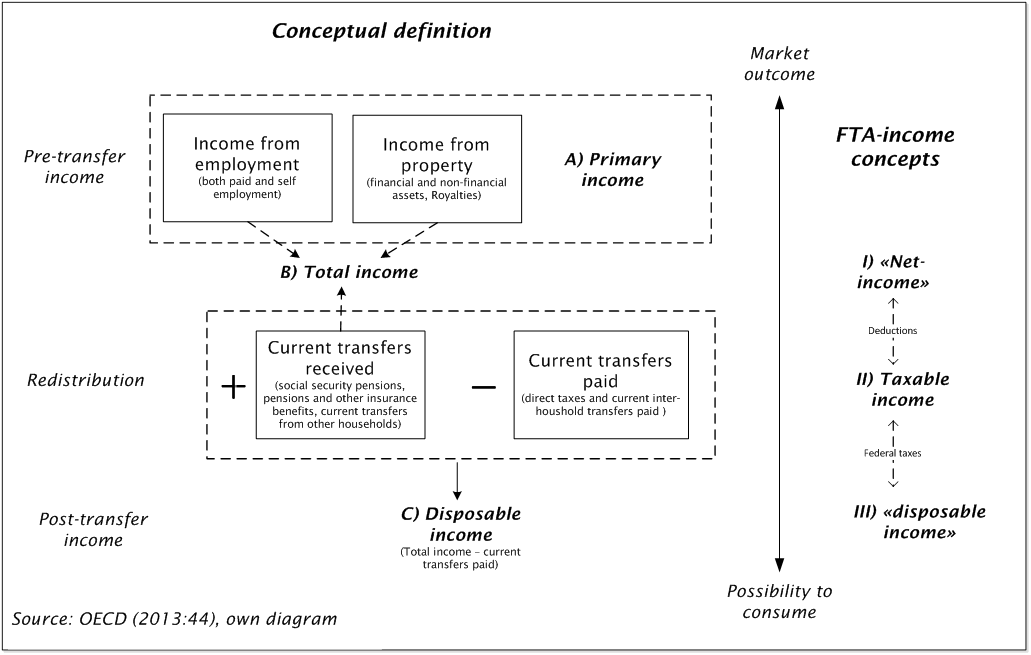
\includegraphics[width=\maxwidth]{figure/income_definition}
\caption{Income definitions}
\label{fig:incdef}
\end{figure}
}

% Quelle zu Abzügen:
% http://www.bilanz.ch/invest/steuern/netto-oder-reineinkommen
% Die rechte Seite mit den Steuergrössen könnte ausführlicher beschrieben werden
% Beispielsweise könnte man zeigen was Nettoeinkommen, Reineinkommen und steuerbares Einkommen sind
% Allerdings steht uns nur Reineinkommen und steuerbares Einkommen zur Verfügung

% ACHTUNG: Wir m?ssen innerhalb des Papers einheitlich bleiben. In der Grafik steht jetzt "Total income" oben steht "Net income"

% Man k?nnte es auch konzeptionell auf kantonale Steuerdaten erweitern. Besser w?re es, dies einfach im Ausblick zu erw?hnen

% Es musse klar werden um was es geht.
% These definitions are contrasted with income concepts, which can be derived out of the FTA tax data.

The central income reported through tax statistics is the taxable income. It includes all reported incomes (income from employment, income from property and received transfers\footnote{Means-tested benefits are not taxed and therefore not included in tax data. Income for low income groups are therefore underestimated. However, \citep{piketty_income_2003} note that non-taxable social security benefits grew as a share of personal income in the US but find that these changes had only a trivial impact on top income shares.}) minus several deductions. It is therefore neither a pre-transfer income nor a post-transfer income measure. It's rather something in between. As the FTA tax statistics include some but not all deductions\footnote{The difference between the real total income and the taxable income are deductions. These include: professional expenses, travel expenses, interest on debt, alimonies, training costs, two-earner deduction, party contributions, private pension provision ``Säule 3a'', buying into the pension plan and sideline deductions} it is possible to calculate a sort of total income, which is called ``net inomce'' (Reineinkommen). As some deductions can be interpreted as compulsory expenses similar to taxes the step towards total income is a step away from the income, which can be used for consumption. Similar when calculating the disposable income out of the taxable income through accounting the reported federal taxes, this is a step towards the income, which is left in the basket for consumption (disposable income). Again it is not a "pure" disposable income, because cantonal, municipal taxes and taxes from churches, which represent the bulk of taxes in Switzerland, are missing.   \\   

% market income mit primary income ersetzen!
% Nicht vergessen: Abzüge können über die Zeit ändern. Was bedeutet das? 

%RF (16.06.2014): den letzten abschnitt finde ich etwas schwer zu verstehen als jemand der nicht tief in der materie ist. vielleicht könnte man sowas machen: It is possible to calculate a kind of "total income" that is in between net and gross income. The principle applied is to only deduct expenditures that are unavoidable.
%OH (16.06.2014): bin mir nicht sicher, ob's mit gross income einfacher ist (kommt in der Grafik nicht vor)


% Allenfalls darauf hinweisen, dass die Wahl der Einkommensdefinition von der Forschungsfrage abhängt. Inequality in market outcome (genderdifferences) requieres to look at market earings from employment, to assess the role of redistribution different steps of income has to be looked at. Following the idea of economic wellbeing usual disposable income is looked at


\emph{Statistical units} \\
The agreed standard on the statistical units, which should be the base of inequality analysis, are households not individuals \citep[60]{oecd_oecd_2013}. Indeed it are individuals, who receive income, own assets and experience economic well-being, but their possibility to do so, is strongly tied to the concept of household. A household comprises all persons under the same housing arrangement. The basic underlying assumption for collecting data on household level instead of individual level is, that people in the same household share resources and therefore pool their incomes (when two or more earners live together) and/or use the household income to provide the essentials of living for every household member (also non-earing members, like children). Additionally, there are economies of scale when people share living space and commodities and they therefore benefit from the sharing. To compare the individual economic well-being among individuals living in different households usually equivalence scales are used (see \citealt[173]{oecd_oecd_2013}, \citealt{buhmann_equivalence_1988}). \\

In tax data, however, the units are represented according to administrative rules. Tax units therefore neither represent individuals in every case nor true households. Tax units rather represent individuals and couples, but couples, who are married or officially registered. This doesn't imply, that those couples live together, as it is needed to satisfy the definition of a household. On the other hand, is it quite likely that more than one tax unit lives in the same household (unmarried/unregistered couples, see \citet[99]{muller_vermogenslage_2014}). It is therefore not directly possible to elicit households and household income from tax data. This might influence the assessment of inequality development, taking into account the change from traditional household and family structures over the last century. \\


% Allenfalls die Br?lhart-Daten erw?hnen und die m?glichkeit der Haushaltsbildung ?ber Abz?ge. Falls wir auch eine Grafik zur Rolle der Haushaltszusammensetzung machen (ich denke schon)
% gibt es studien? Zur Bedeutung von ?quivalenzskalen und zur Bedeutung der Differenzierung von Haushalten und Individuuen?
% inequality and family structure> review ny (McCall & Percheski (2010))
% Was ist zu erwarten, wenn Äquivalenzskalen vernachlässigt werden? Soll man dies erwähnen oder einfach weglassen

\emph{Measuring inequality or concentration} \\
To be able to make qualifying statements about a distribution or to compare different distributions, the concept of inequality turned out to be the most appropriate and thus the most commonly used dimension. The Gini coefficient is the most known measure and mainly used for international comparison. As it is derived from the Lorenz-curve, the quantified amount of inequality can unpretentiously be described in a formal and visual way. Therefore the Gini coefficient is easily interpretable. Furthermore it has several desired statistical properties \citet{engelhardt_modelle_2000}. (1) ``\textit{principle of population}'': the assessment of inequality is independent of the population size (2) ``\textit{Requirement of Bresciani-Turroni}'': the measure is sensitive for changes of income shares, but not for absolute changes (e.g. doubling of all income) (3) ``\textit{weak principle of transfers}'' or ``\textit{requirement of Pigou-Dalton}'': transfers from richer households lead to a reduction of inequality. However, several drawbacks are reported in the literature. The most important point is, that the underlying distributional form of the measured inequality is unknown and it is therefore not possible to see if the measure is driven by a few rich or many poor individuals. This can also be problematic for comparison between countries or over time. In extreme cases two totally different distributions share the same Gini-coefficient.\\

% namen mit principle ergänzen?

The recent wave of tax-data studies do not report Gini-coefficents. Rather top income shares are informed on, which are calculated not only with tax data, but corrected using marginal distributions of income and population using external sources (census data and national accounts). This procedure ensures, that the inequality measure is not biased because of non-fillers, who do not appear in tax statistics.  \citet{leigh_how_2007} compares top income shares with other inequality measures and asks, whether they are a useful measure of inequality in a society. He tries to answer this question empirically by comparing measures of inequality based on top income shares with measures of household or family inequality. He finds a strong positive relationship, but concludes (P.600): ``top income shares are far from perfect as a measure of distribution of income across society.'' Top income shares hence inform not completely on how inequality evolves elsewhere in the distribution. Furthermore, top income shares only weakly satisfy the Pigou-Dalton transfer principle (in contrast to the Gini-Coefficent as mentioned above). A transfer from rich to poor will indeed never increase the top income shares, but if the transfer is between individuals, who are either both within the top group or both outside the top group, then the share measure will remain unchanged. \\

% Auf deutsch würde ich noch ebd.

Newer branches of inequality studies emphasize the need for broader measures of inequality, which allow more detailed analyses about the change of inequality and namely statements about the area of change (downgrading/upgrading). The polarization index developed by \citep{handcock_relative_1999} is capable of doing this. Recently this index was applied in the work of \citep{alderson_exactly_2005} and \citep{gornick_how_2013}. This approach is rooted in relative distribution methods. It includes a precise comparison of the shape of two distributions (groups, over time). As the main advantage this approach allows to characterize the change in detail. It is possible to see which parts of the distribution changed, e.g. whether a polarization occurred (reduction of middle class) -- which equals an increase of inequality -- or this change is driven by either a change in the upper or lower part of the distribution.  \\
 
The literature mentions several other metrics with desired properties we will not discuss here (see for example \citet{cowell_chapter_2000} and \citet{hao_assessing_2010}).\\

% Allenfalls auch auf Quintilvergleiche eingehen und Atkinsonmass 


\emph{Population Coverage}
% beim letzten Punkt geht es um Steuerhinterziehung. Fällt das auch noch unter Population coverage?
 
Often inequality is assessed on national level, which implies, that studies try to cover the whole population of the country of interest. This is a special thorny task for surveys working with samples, because nonresponse is a major source of bias \citep{bethlehem_handbook_2011}.  \citep{korinek_survey_2006} show, that the position in the income distribution influence the probability to participate in a survey. Low income and high income households are more likely to refuse survey response, which leads to an overrepresentation of middle income households. This process can be referred to as the "middleclass bias" \citep{diekmann_empirische_2009}. Missing data in household surveys is therefore not missing at random, which has an impact on the measures of inequality. The magnitude of this bias in Switzerland, however, is unknown. Strategies to handle this kind of bias are discussed in the literature \citep{sarndal_model_2003}, but require a register for every unit, that is proportional to income. Currently no such register exists for Switzerland \citet[43]{muller_vermogenslage_2014}. Currently used micro datasets, which are used for official publications concerning inequality in Switzerland (SILC and HABE) are furthermore confronted with a constructed coverage problem, because these surveys rely on the phone register, which excludes households not having a registered connection. \\
%(Problems of collective households, ecoplan 2014:45). Erw?hnen?

The issue of incomplete coverage is less dramatic with tax data. Essentially every permanent resident in Switzerland over 18 years of age (respectively 20 years of age prior to 1996) is taxed on a yearly base (or every two years before the change of the tax system). Basically this leads to a full representation of the adult population of Switzerland and a complete coverage of the income distribution. This includes a separation of normal cases, which embrace the majority of taxpayers, and the special cases, which cover (not only) foreign nationals living in Switzerland but with a yearly or any other temporary resident permit only. Most important this includes high net wealth individuals taxed according to their expenditures. Special attention has to be paid to tax units with none or very low incomes. Even though they have to hand in a tax return, their income does not show up in the statistics if their income after deductions falls below the threshold (e.g. CHF 16.900 for singles in 2010) and they are therefore not taxed with direct federal taxes. This is possible for normal and special cases alike. From 1995/1996 until 2010 the number of non-taxed units is reported, but not for the years before. Dell et al. (2007) try to estimate the fraction of non-taxed by comparing the reported numbers of tax units to census reports about the number of adult population. According to their estimations this fraction drops from 94\% in 1993/1994 to 63\% back in 1945/46. \\

Another critical issue with tax data is the problem of tax evasion, which definitely can bias the assessment of inequality. \citet{alvaredo_income_2009} for example regard estimates of Spanish top incomes prior to 1981 as unreliable due to widespread tax evasion. Evasion can occur, when individuals try not to fill tax returns or by misreporting of incomes. In Switzerland non-fillers show up in the tax-statistics either way, as long as they are registered. This person gets an imputed income based on an older tax return and information given by employers. Only non registered non-fillers are not in the records. Therefore non-fillers are a minor problem. Not negligible is the circumstance, that individuals misreport incomes. \citet{feld_tax_2006} examine the role of tax evasion in Switzerland by calculating the difference of the national accounts measures of primary income and the income reported to the tax authorities. They can show, that the average level of income tax evasion from 1965 to 1995 varies between 13\% and 35\%. They suggest, that evasion is heavily driven by capital income tax evasion. \\


\emph{Comparison of tax data and other data sources - advantages and shortcomings}

Based on this sections previous discussion table~\ref{datacomp} summarizes important differences between tax and survey data related to analyses of income inequality. 

% Suitability of data sources can be judeged by different criterias. crossectional or longidutional perspective. longidutional perspective allows for dynamic 

%[ich stelle mir eine Tabelle mit verschiedenen Dimensionen vor, anhand derer eine Einordnung unterschiedlicher Datenquellen geschieht.]
% Mögliche Vergleichsdimensionen
%- Suitability of cross country comparison
%- Coverage of the population of interesst
%- Implementation of common concepts of economic ressources
%- intertemporal comparision
%- flexibel applications of appropriate inequality measures
% - appropriate income definition

\multicolinterrupt{
\begin{table}[H]
\caption{Comparison of tax and survey data\label{datacomp}} 
\begin{center}
\begin{tabular}{lcc}
\hline\hline
                                   & Tax data       & Survey data\\
\hline
Statistical unit                   & tax units (individuals/married couples)  & households\\                                   
Concepts of economic resources  & data-driven   & theory-driven\\
Population coverage & total population & sample \\ 
Top incomes covered                 & yes   & no\\
Low incomes covered?               & no        & yes\\
Comparison over time possible 	   & long       & short \\
Cross country comparison possible? & limited   & possible\\
\hline
\end{tabular}
\end{center}
\end{table}
}
%RF: damit haben wir WER, WANN, WAS, wollen wir noch ein WOMIT/WAS DARSTELLEN -> methodik -> reldist ? jaa


To define a standard of measuring economic resources and related inequality we discussed different dimensions of demands the data needs to meet. To sum up, ideally we want to measure \textit{disposable income} for \textit{all} swiss \textit{households} yearly for an extended period of time. Tax data has one weakness when it comes to the ideal income measure as we need to work with ``taxable income'' which is designed to serve taxation purposes. However, both concepts -- what needs to be taxed and what can be spent -- are related as both address a distinction between necessary and voluntary expenses. By subtracting federal taxes from taxable income we are getting closer to the theoretically ideal income measure of disposable income. However we can not subtract the more important cantonal and communal taxes. 
The second most important drawback with tax data is that it does not adequately address households. There are few situations in which the tax unit equals the household, that is for individuals living alone, with married partner and/or deductible children and nobody else. This ``classic'' household setup however became less common in the last decades so we need to assume statements about household inequality based on taxed data became more and more biased. 
%The swiss law seems to be slightly outdated in this context.
Finally however, another advantage of tax data (over survey data) is indeed the observation period. While the FTA data we use range back to 1945, the earliest period of survey data is 2000 (HBS data). The striking feature of the long FTA time series is its consistency. Both population coverage and income measures are rather consistent for the complete observation period\footnote{Limitations might however exist due to tax evasion and major changes in the tax system, e.g. 1945. Furthermore, tax units with incomes too small to quality for federal taxation are not documented before 1995 and treated as zeros afterwards making it difficult to track income development in the lower percentiles.}. This can not be said for survey data as these are based on samples and therefore require an ideal sampling design or reweighting to be representative and comparable over time. We will see how well sampling and weighting is done in the results section.


% Braucht es alle drei Survey-Befragungen
% ich würde nicht dichotomisieren, sondern ordinal bewerten (tief, mittel, hoch)

% Die Punkte kurz beschreiben.
% Zusammenfassung


% Gedankenstütze
%\textbf{Problems with household income surveys}
%\begin{itemize}
%\item Sample data (bias)
%\item comparability between countries and over time (depends on income definition)
%\item short time series
%\end{itemize}


%Burkhauser et al. (2009) compare inequality statistics form survey data and tax records to consolidate the findings about recent trends in the USA
%Studies on problems with survey data See for other countries: \citealt{Siminski et al 2003 FEHLT} (Australia), \citealt{Brewer et al 2008 FEHLT}, UK, \citealt{Burkhauser et al. 2009 FEHLT}, US)


%Warnings about the use of tax data
%The use of tax data is often regarded by economists with considerable disbelief. These doubts are well justified for at least two reasons. The first is that tax data are collected as part of an administrative process, which is not tailored to the scientists' needs, so that the definition of income, income unit, etc., are not necessarily those that we would have chosen. This causes particular difficulties for comparisons across countries, but also for time-series analysis where there have been substantial changes in the tax system, such as the moves to and from the joint taxation of couples. Secondly, it is obvious that those paying tax have a financial incentive to present their affairs in a way that reduces tax liabilities. There is tax avoidance and tax evasion. The rich, in particular, have a strong incentive to understate their taxable incomes. Those with wealth take steps to ensure that the return comes in the form of asset appreciation, typically taxed at lower rates or not at all. Those with high salaries seek to ensure that part of their remuneration comes in forms, such as fringe benefits or stock-options which receive favorable tax treatment. Both groups may make use of tax havens that allow income to be moved beyond the reach of the national tax net. These shortcomings limit what can be said from tax data, but this does not mean that the data are worthless. Like all economic data, they measure with error the 'true' variable in which we are interested.
%The data series presented here are fairly homogenous across countries, annual, long-run, and broken down by income source for several cases. Users should be aware also about their limitations. Firstly, the series measure only top income shares and hence are silent on how inequality evolves elsewhere in the distribution [why?]. Secondly, the series are largely concerned with gross incomes before tax. Thirdly, the definition of income and the unit of observation (the individual vs. the family) vary across countries making comparability of levels across countries more difficult. Even within a country, there are breaks in comparability that arise because of changes in tax legislation affecting the definition of income, although most studies try to correct for such changes to create homogenous series. Finally and perhaps most important, the series might be biased because of tax avoidance and tax evasion. For the details, we refer users to the original papers (see also Atkinson, Piketty and Saez, 2011).




\section{Methods}


% Diese Abschnitt muss ersetzt werden mit der von uns gewählten Vorgehensweise

In the last section we described the advantages and drawback of tax-data discussing five aspects, which we regard as crucial concerning the assessment of inequality. To get a feeling of the importance of these aspects, we exploit the FTA-tax data as far as possible and perform several insightful calculations addressing four of the five mentioned aspects. No further investigation is possible regarding aspect (1) concepts on measuring economic resource. But for the other four thematic areas, we can provide deeper insight. In general our main strategy is to apply different possible concepts within one conceptional area (income, units, measurement, population coverage) while holding other conceptual differences constant. With this strategy we want to show, the sensitiveness the assessment of inequality is especially if one looks at time trends.\\

To fulfill the above described task, we use two techniques. To assess the development over time, we calculate in general Gini-coefficients for all possible time points, allowing us the make time trends visible and to compare the result out of the FTA-tax data to other publications. For selected periods we expand the analysis with relative distribution methods, which allows an in-depth analysis of distributional differences and therefore catches the shortcomings of Gini-coefficients. \\

To calculate Gini-coefficients we follow common definitions, like it is described for example in \citep{jann_einfuhrung_2005}. Because the relative distribution methods are not that widely known, we provide a short introduction of the important concepts in this section. We additional expand the method section with an extended analysis about the importance of non-taxed, because the issue of non-taxed is a especially thorny one.


\subsection{Relative distribution (RD) framework}

The RD-framework is based on the concept of a ``relative distribution'', a transformation of the data from two distributions into a single distribution that contains all of the information necessary for scale-invariant comparison. This allows to make distribution differences ``visual'' in an elegant way and it is also a base for summary statistics, which are more sensitive to detailed theoretical hypotheses in contrast to other measures like the Gini-coefficient or top income-shares, which inform either about the whole population or only about the top part of the distribution.\\

% Probability Density function as a base for the RD
The goal of RD is to study the differences between two distributions. A common example could be the income distribution for man and women. Subject of the comparison can also be two distributions describing the same population, but stemming from two different data sources like survey or tax data or even comparison of the same source/population but for different time points, like the income distribution out of tax data for Switzerland today compared to an earlier time point. To describe how the two distributions are gone be transformed into a relative distribution, we start with defining the two distributions. One represents the reference population $Y_{0}$ and the other the comparison population $Y$. $x$ represents our measure of interest (income). A first visual approach is to compare the two probability density functions (PDF). The PDF is a function $f(x)$ which describes the distribution of probability over the outcome set and is defined for all possible values of $x$. This function integrates to 1, which means that the sum of all probabilities over all possible values is 100\%. Out of the comparison of the PDF, it is possible to see, which values of $x$ are more and less probable. This already allows to spot distributional differences over the whole scale of $x$ visually. \\

The PDF can be characterized by its cumulative distribution function (CDF). The CDF can be formulated as $F(x)$, which represents the probability that a randomly chosen value is less than or equal to $x$. The relative distribution of $Y$ to $Y_{0}$ is then defined as 

\begin{equation}
R=F_{0}(Y)
\end{equation}

$R$ is obtained from $Y$ by transforming it by the CDF for $Y_{0}$, $F_{0}$. $R$ therefore measures the relative rank of $Y$ compared to $Y_{0}$. 

% Relative Distribution


\begin{equation}
g(r)=\frac{f(F_{0}^{-1}(r))}{^{f_{0}(F_{0}^{-1}(r))}}
\end{equation}


We can calculate the Probability Density Function $g(r)$ of R, where $r$ represents the proportion of values and $F_{0}^{-1}(r)$ is the inverse cumulative distribution function, also called the quantile function. $g(r)$ can be interpreted as a density ratio, which is defined as the ratio of these two quantities evaluated at every percentile of the reference distribution [0,1]. With a complete overlap of both distributions the probability density function of the $R$ is 1 at every point of the PDF. On the other hand, values higher than 1 represent higher probabilities in the comparison distribution than in the references distribution at this specific point and values lower than 1 respectively represent lower probabilities. It is a proper PDF in the sense that it integrates to 1 over the unit interval.\\

% Median and shape differences
What we got through the above transformation of two distributions is the overall relative probability density. But differences between distributions can be divided into two basic components: changes in location and changes in shape. If the comparative distribution is a simple location-shifted version of the reference distribution, then the difference between the two distributions can be parsimoniously summarized by this shift. Differences that remain after a location adjustment are differences in ``shape'' (scale, skewness and other distributional characteristics). When both types of shifts are operating, or when factors other than scale are changing in the shape component, we need a way to separate out the various effects. If we want to identify the effect of a location shift and separate it from other changes in the distribution, it is necessary to specify what scale this shift operates on. It is possible to adjust distributions by any measure of central tendency. Here we choose a median location adjustment because the median is a natural, robust and scale invariant unit of measurement. Because our interest lies in analyzing distributional differences concerning the degree of inequality, we will focus in the results section on shape differences and look therefore at the relative distribution after the distributions are adjusted for location differences. 

% R based Summary Meausres
Distributional polarization is of particular interest in the study of inequality. However, common inequality indicators (for example Gini or Theil’s index) are not designed to distinguish between growth in the upper and lower tails. Even if the measures register increasing inequality over time, one cannot distinguish a polarization of the distribution (increases in both tails) from upgrading (increases in the upper tail) or downgrading (increases in lower tail). The polarization index developed by \citep{Handock and Morris 1999} addresses this issue, because it is decomposable to distinguish differences in the upper and lower tails.  Because it is based on the relative distribution it provides a simple link between what is observed in the graphical display and what is measured by the numerical summary. \\

The median relative polarization index (MRP) is defined as the mean absolute deviation around the median of the location-adjusted relative distribution, scaled to produce an index that varies between -1 and 1. Given the scaling, a value of zero represents no differences in distributional shape; positive values represent more polarization (increases in the tails of the distribution); and negative values represent less polarization (convergence towards the center of the distribution). The measure catches only differences in distributional shape (not location). And it has several interesting features. MRP can be interpreted in terms of a proportional shift of mass in the distribution from more central to less central values. A value of 0.1, for example, is equivalent to a 10\% population shift from the center of the distribution to the upper and lower quartiles and the MRP is decomposable along the scale of $y$. This makes it possible to compare the contribution of each section of the distribution to the overall polarization. A natural decomposition is the contributions made by components above (upper polarization index, URP) and below (lower polarization index, LRP) the median (of $g(r)$).


%%%
% Was soll hier beschrieben werden und was direkt bei den Tabellen?
%%% Gar nicht so einfach....

%%% Nach Lehrbuch müssten die methodischen Schritte hier beschrieben werden.
% Man könnte zu den Zeitreihen jeweils die Varianz ausweisen-> dass würde helfen die Reihe zu beurteilen. Man sieht dann: aha, die Reihe ist im Vergleich zur anderen höher/tiefer. Ob die Reihen stärkeren Schwankungen unterliegen könnte einfach aus der Varianz gelesen werden


% Defining income
% Beschreiben, dass sich aus den publizierten Einkommensgrössen und den Steuerbeträgen unterschiedliche 
% Einkommen berechnen lassen
% Es steht der Vorwurf im Raum, die unteren Einkommen seien mit Steuerstatistiken schlecht abgebildet, weil bedarfsabhängige Leistungen nicht versteuert sind

% Es müsste eine Reihe zum gesetzliche Grundbedarf vorliegen. Wüsste ich jetzt grad nicht von wo...

%%
% statistical units
% Beschreiben, dass zwar keine Haushaltseinkommen gebildet werden können und Skaleneffekte nicht abgebildet sind, dass eine Annäherung jedoch möglich ist
% Definition der äquivalenzskala bei Brülhart (korrespondiert nicht mit OECD Definitionen, aus pragmatischen Gründen)

%%
% Measuring inequality
% Beschreiben, wie sich aus gruppierten Steuerstatistiken der Gini-Koeffizient berechnen lässt
% Beschreiben wie wir relative distribution technics einsetzen und den Polaritätsindex berechnen

% Calculate the gini
% Ein bisschen erklären, wie aus gruppierten Tabellen der Gini-Koeffizient berechnet wird.

% Polaritätsindex
% Alderson and Doran (2013:56) beschreiben zwei mögliche Indizies Median relative polarization index (MRP) eingeführt von (Morris, Bernhardt und Handcock 1994:217), der in den lower relative polarization index(LRP) und den upper relative polarization index (URP) zerlegt werden kann (ebd.209)
% (1. Schritt) Probability density functions
% (2. Schritt) Overall relative density function -> Achtung diese Dichtefunktion bildet sowohl die  Lokationsverschiebung als auch durch Verschiebung der Form ab. Eigentlich interessiert aber, der shape shift
% Deshalb wird die Verteilung um die Lokationsverschiebung bereinigt und nur der shape-shift angeschaut. Ausgewiesen werden (MRP)-> hat polarisierung stattgefunden: LRP und URP-> ist polarisierung eher auf eine Zunahme armer (LRP) zurückzuführen oder auf eine Zunahme von Reichen? (URP)


%%
% Population coverage
% Analysen zu den Nullern > ist eine Hauptkritik an der Nutzung von Steuerdaten
% Die Bedeutung von Normal- und Sonderfällen
% Den Vergleich mit der HABE beschreiben, welche Einkommensgrösse nutzen wir aus der HABE um diese möglichst mit den Steuerdaten vergleichbar zu machen? Wir brauchen das Bruttoeinkommen nach Abzug der Sozialversicherungsbeiträge, dies lässt sich mit dem Reineinkommen vergleichen




%%
% Intertemporal comparison
% Ziel eine möglichst lange Zeitreihe abzubilden. 
% Technik der Lückenfüllung von Ben beschreiben> dies kurz anderen Techniken gegenüberstellen.
% Konfidenzintervalle für die Perioden mit vielen fehlenden Werte?

% eine / oder zwei Zeitreihen (eine lange und eine, die möglichst nahe an der richtigen Konzeptionalisierung ist: post direct taxed income, normal+sonderfälle) zusammen mit den bereits existierenden Reihen (HABE,LIS,SILC) ploten



%\textbf{Incomplete coverage of the population (left censored data.)} What can be done about the not-taxed? \citet{dell_income_2007} impute for non-fillers the 20 percentage of the annual average income. This flattens the distribution on the left side, which is not a problem if you are interested in the top income shares, but it would surly affect overall measures of inequality. Furthermore the authors calculate the proportion of non-fillers by estimating the total of tax units out of the population records. \\

%\textbf{changes in taxation system  (switch from annual to biannual taxation)} In the mid-1990s a fundamental change in the Swiss tax system took place by switching form the two-years based praenumerando taxation to the one-year based postnumerando taxation. This change was enacted with a transitional period of several years, during which each canton could choose when to adopt the new system.  This is why during the transitional period from 1995 to 2003 there is no uniform tax data published on the Swiss level but only data on the cantonal level \citep[8f]{foellmi_volatile_2013}. \\
%es wird erwartet, dass der Wechsel Ungleichheitsmasse beeinflussen. Yearly fluctuations are dampened, when income is measured on a two-yearly basis.

%\textbf{Estimating percentiles from bracket income tabulation} Pareto interpolation \\ 

%\textbf{Missing of mean-tested benefits as part of the income} -> imputation with recommendation for minimum level for basic needs defined by the SKOS.\\
%is never mentioned as a problem, but it seems to me a better way to approach the non-taxed issue, than dell way (20 % of average income)
% Beim Imputieren m?sste man auch die Zahl der freiwilligen Nichtbeziehenden ber?cksichtigen.

%\textbf{deductions} \citet[477]{dell_income_2007}:" we can check with statistics for 1971-72 (as well as later years) presented both by size of income before deductions and income after deductions that adding back deductions does not introduce any significant error in our estimates."
%\citet[5]{schaltegger_evolution_2011}: ``..., information on [...] deductions is provided in the tax statistics, thus, we could add the personal deductions to the income data to obtain a consistent series over time''. Können wir das auch? Zumindest für gewisse Zeiträume? Das wäre noch gut. \\

%Studies on income try to focus on the disposable income, which subtracts certain expenditures from the primary income. Deductions reflect somehow compulsory expenditures and thus taxable income can be seen as a sort of pseudo disposable income. On the other hand deductions can affect the distribution. There are recent studies about the correlation of progressivity and deductions in Switzerland, which examines if deductions have a ``perverse redistribution'' effect by redistributing income from the lower middle class to the upper middle class (see \citealt{peters_steuerabzuge:_2011} and \citet{Interpellation Barbara Gysel (2009) FEHLT. das interpellation barbara sieht falsch aus}.

% Income share specific problems
% Total income denominator Exogenous Approach -> net income reported in the national accounts. Endogenous Approach -> Dell et al. technic-> imputing 20\% of average personal income to non-fillers (which are mainly persons with low or no income). Honestly , is this appropriate? (Everyone did it)
% Total of tax units in the country. exogenous approach -> construct number of total tax units artificially from other data sources
% Endogenous approach -> reported in the tax tables 

%%%-------------------------------------------------%%%
%%% Abschnitte aus ersten Version des Papers %%%
%%%-------------------------------------------------%%%

%\subsection{Hypotheses}
%Based on the theories we test the following hypotheses:

%\begin{itemize}
%\item H1: Develpment of inequality is driven by sectoral change
%\item H2: Development of inequality is driven by political change, i.e. economic crisis contribute to inequality because welfare states tend to be downsized
%\end{itemize}

%\subsection{Data and Variables}

%We use data from the Swiss Federat Tax Administration (FTA) where our data about incomes ranges from the years 1941/42 to 2010. While the data results in a long and consistent time series to illustrate swiss inequality development, there are a few pitfalls we want to adress which might be of interest for other research on this topic (be it in Switzerland or other countries).

%\subsubsection{Left censored data}

%The FTA provides data about all tax units in Switzerland that are liable to pay federal taxes.A tax unit may be a single person or a household. The taxable population however is not identical to the population which should be used to calculate measures of inequality. Precisely, the data do not contain tax units with very little incomes so calculations based on these data treat the lowest percentiles equally to tax units with zero income.Figure X shows the threshold to be hit to enter the statistic.

%\textcolor{red}{[FIGURE X ABOUT HERE] soll zeigen: Zeitreihe der Untergrenze von 1941-2010}

%So first of all, there is a bias in the level of an inequality measure one could calculate with the   FTA data. Furthermore, also the changes over time might not be interpreted savely as over time the number of tax unit within this "hidden range" might vary or might even have a certain trend. We will adress this issue in detail in the methods chapter.

%\subsubsection{Different measures, different populations}

%The FTA data makes two kinds of distinctions. First, data was collected for so called "normal cases" and "special cases", i.e. a "normal case" is a taxable (for the complete tax period) person or household domiciled in a swiss canton without income from outside of Switzerland. A "special case" therefore is a diffuse reference category that contains tax units that are taxed at source, were not taxable for the complete tax period or generated additional income in another country. Second, the FTA reports two measures, that is taxable income and absolute income \textcolor{red}{(meine vorläufige Übersetzung von Reineinkommen)}. Absolute income is the sum of all incomes (earnings, interest income, rental incomes) minus expenses (e.g. from self-employment or credit cost). The taxable income is calculated as the difference of absolute income and deductions (e.g. children, insurance rates). The longest consistent time series exists for the taxable income of normal cases. So all statements we make with our data only apply to this subpopulation.

%\subsubsection{Changes in taxation and measurement}
%The swiss tax system is highly federal. That means, communities raise taxes which then go to the communities, the canton and the state. If we want to calculate overall swiss measures, we need to take into account, that cantons vary (between cantons and over time) with regard to the tax deductions that are possible and also the mechanism how taxes are collected. The latter adresses a comprehensive reorganization of the swiss tax system where between 1995 and 2003 cantons changed from taxing the past two years of income (postnumerando system) to taxing the present single year (praenumerando system). For details see \textcolor{red}{Martinez (xxxx) or some other author (xxxx)}. Aggregate measures of inequality therefore have to be estimated for the periods 1995 to 2003 which we adress shortly in the methods chapter.

%\subsection{Methodology Used}
%There are two steps of data analyses which need to be described to the reader. First, the estimation of the bias we introduce by estimating measures of inequality when tax units with too little income are not observed. Second, the steps undertaken to estimate aggregate swiss measures by imputing taxable income for those cantons and periods where the change of the tax system produced a gap (1995 to 2003, depending on the canton). 

%\subsubsection{Imputing the gap}
%The imputation is not a focus of the paper so we basically follow the most simple approach of Martinez (xxxx). That is estimating the missing taxable income statistics via OLS using information from time trends and cantons. Our imputation model therefore includes canton inequality measures and periods dummies to explain aggregate swiss inequality.

\subsection{Non-taxed}
Some tax units are missing in the FTA data as they do not qualify for taxation below a certain income threshold. The income distribution is therefore cut at the left end. For most of the observed range it is not documented how many tax units fall into this unobserved category. Since 1995 however the FTA provides the number of people not being taxed (we will call these tax units ``zeros''). From 1995 to 2010 we can therefore estimate the bias we introduce when ignoring the zeros. In this section we will try to analyze whether the bias is stable over time (and cantons). If the bias was stable over time, we could still analyze trends and changes of inequality no matter how severe the bias is. 

First it is useful to look at the descriptives plotting the share of zeros over time.



\begin{knitrout}
\definecolor{shadecolor}{rgb}{0.969, 0.969, 0.969}\color{fgcolor}\begin{figure}[H]

\includegraphics[width=\maxwidth]{figure/zero_descriptives} \caption[Share of tax units below federal tax liability threshold]{Share of tax units below federal tax liability threshold\label{fig:zero_descriptives}}
\end{figure}


\end{knitrout}

The number of zeros increased slightly according to figure \ref{fig:zero_descriptives}. Different interpretations seems possible. The increased share of zeros could be driven by the FTA's inflation adjustments or an increase in social deductions. Another plausible explanation is the increasing number of unmarried couples filling in two separate tax forms instead of one so we observe two ``small'' incomes instead of one ``large'' income, thus inflating the number of people falling below the taxation threshold. 

%\begin{enumerate}
%\item There is a small overall upward trend which we assume to be the Federal Administrations inflation adjustments to the tax threshold.
%\item Geneva and Tessin show wild changes but those might be explained by the tax gap ("Bemessungslücke") that people exploited when the cantons changed the tax system. It %remains unclear however why we can't see similar patter within other cantons.
%\item There is some variance and we see different patterns over time and cantons. When estimating Gini coefficients or the like we must therefore assume that ignoring ``the zeros'' leads to a bias that is not stable over time.
%\end{enumerate}

As we want to report reliably inequality time series we pursue two strategies:

\begin{enumerate}
\item Add the zeros as a separate group
\item Carry out a statistical test whether the share of zeros alters the Gini coefficient
\end{enumerate}

By adding the zeros back as a separate group we need to make an assumption about the income distribution within that group. We know these cases had incomes between zero and the threshold (usually around 15.000 CHF for the period 1995-2010). In figure \ref{fig:with_without_zeros_Gini} we show Gini-coefficients calculated under the assumption of the zeros being zero. This is problematic for two reasons: first we know these units might earn more (up to the threshold) so Ginis calculated on this assumptions will be too high. Second we assume the zero group to be perfectly homogeneous which on the contrary has a lowering effect on the Gini coefficient. Therefore we must at least assume a distribution for the zeros that has some variance and ranges from zero to the threshold. We decided to use the most simple approach fulfilling both criteria which is to interpolate a uniform distribution between zero and each tax periods threshold.

The second approach investigates whether the FTA time series is suitable to analyze trends of inequality even if the inequality measures are biased. We can do this by regressing the inequality measure (here the Gini-coefficient) on the share of zeros. Simply spoken we test if cutting a larger (left) tail of the distribution changes the shape of the distribution. We include Gini-coefficient for all cantons in our analyses to improve the power of our statistical test\footnote{Furthermore without cantonal data (but only data for aggregate Switzerland) it is impossible to distinguish whether inequality changed due to the number of unobserved people or any other variable that changed over time)}. 

\begin{knitrout}
\definecolor{shadecolor}{rgb}{0.969, 0.969, 0.969}\color{fgcolor}\begin{figure}[H]

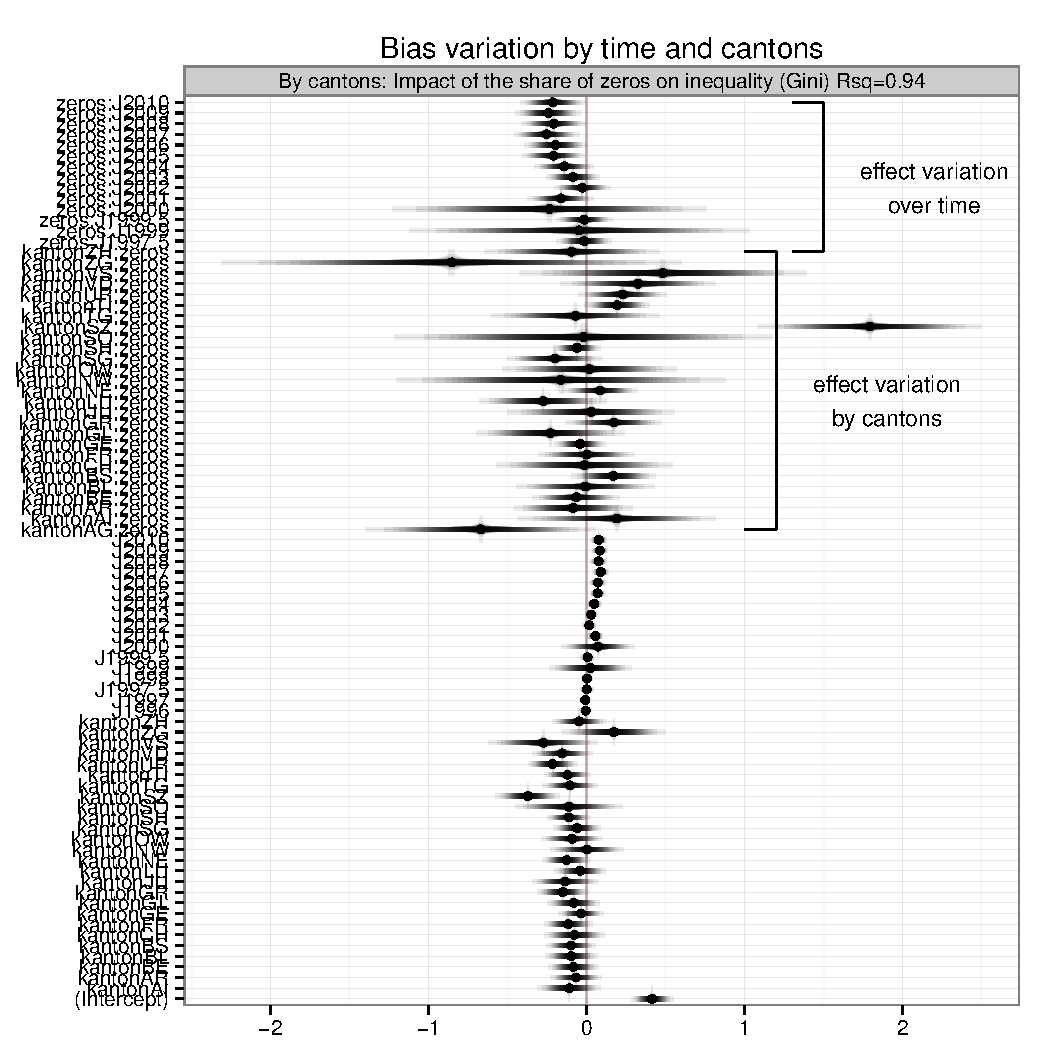
\includegraphics[width=\maxwidth]{figure/corrected_gini} \caption[Bias variation by time and cantons]{Bias variation by time and cantons\label{fig:corrected_gini}}
\end{figure}


\end{knitrout}

The model outputs a test statistic for each canton that tells us whether the variation of the zero-rate over time leads to a significant deviation from the typical ``canton gini-level''. As the model has a decent fit we are not in great danger of omitted variable bias. Using a joint F-Test we can now test if all canton interactions are zero. 



In our case we can clearly reject the hypothesis that all interactions are zero ($p=0$). This leads to the conclusion that Gini coefficients are biased by the variation of the zero-share. As a minimum a researcher using tax data should therefore control the share of unobserved people, while the best solution is to thoroughly the mechanisms behind a change in the zero share (e.g. this might be due to increased unemployment in one period and due to changes of the tax system in another period.). Fortunately the model coefficient of Switzerland as a whole is not significant suggesting that the cantonal biases cancel each other out. This seems plausible if the phenomenon is e.g. driven by tax competition because most of the ``tax optimization'' happens within Switzerland.
% which is kind of obvious but at the same time we can use the model to report adjusted Gini coefficients. For example one might be interested in how inequality would had developed if the zero-share would have been constant over time. (Note RF: predict all data point using canton, time and the initial OR final zero-share to homogenize the time series)
%Furthermore we can quantify how large the bias is and we can do this separately for tax periods or separately for cantons. 

%For all cantons:

%<<magnitude_of_bias>>=
%reduced_fit <- lm(G_steink~kanton+factor(steuerperiode),data=df)
%#summary(reduced_fit)
%@

%We can see the the model fit reduces to explaining 61.5\% of the Gini variation versus 92.6\% when the information from the zero-shares was used. Although this so some extent attributable to the additional 26 parameters: this is huge. 

%The model indicates some cases that deserve more attention: Schwyz (positive coefficient) and Geneva (negative coefficient) and the tax period 2000 as well as the most recent periods.

Figure \ref{fig:corrected_gini} can be read as follows: A positive coefficient (e.g. Schwyz) states that we measure higher Gini coefficients in periods with many zeros. We can derive, that the distribution of incomes is more skewed for high incomes than for low incomes. Simply speaking, the contrast between low and middle class is less pronounced than the contrast between middle and top class. One possible explanation would be that incomes stem from two different distributions (populations): 1) local people of Schwyz who follow a less skewed distribution and 2) particularly rich people who moved to Schwyz (to avoid taxes). 

A negative coefficient (e.g. Geneva) means the more zeros there are the smaller the Gini measure was compared to other tax periods within that canton (remember this is a fixed-effects model). This is the case we would usually expect: more zeros mask inequality that arises from the bottom.

Another information we can read from the coefficient plot is the (zero-)adjusted inequality development represented by the period dummies. However these values indicate an unweighted change of the Gini coefficient which relates to cantons (not aggregate Switzerland). Fortunately the overall picture of inequality development looks very similar to the plain time series of Gini coefficients. 
%What can we conclude from that analysis? First one must notice that aggregate measure like the Gini (or others) do not always react in the same way when we cut off one part of the distribution, therefore the measures calculated from tax data is biased. On the other hand, the model coefficient of Switzerland as a whole is not significant suggesting that the cantonal biases cancel out each other. This seems plausible. Most of the ``tax optimization'' happens within Switzerland so the rich people who moved to Schwyz are now missing at another canton.

And there is even more to see from the model coefficients: The period-zero-interactions in the model state how an increase of zeros (cutting off a larger piece of the left tail) affects the Gini coefficient in each period compared to 1995. We can see that 2004 to 2010 the (negative) effect is significantly larger than 1995. To simplify: cutting off zeros increasingly leads to an underestimation of inequality measures, probably because the skewness in the left part of the distribution increased. To simplify: in the last decade tax units are increasingly pushed below the observable threshold concealing part of the inequality development. One less dramatic interpretation of this result is the increasing number of unmarried couples filling in two separate tax forms.




% Alter Textbaustein zu Vermögen
%\emph{Defining wealth}
%While the apropiateness of the conceptualization of income is widely discuded, there is no agreed definition of personal wealth yet and the appropriate methods of valuation are not always clear. Wealth can be defined as the marketable value of financial assets plus non-financial assets (housing and land) less debts (Credit Suisse 2011:5).

%The discussion about problems with reporting income is fairly exhaustive. What about wealth?

%It is well recognized that the traditional sources of wealth distribution data are unlikely to provide an accurate picture of wealth ownership in the top-tail of the distribution. \citet{credit_suisse_global_2011} makes use of the information in the ``Rich Lists'' published by Forbes Magazine to adjust the wealth distribution pattern in the highest wealth ranges. \\

%Additionally the Credit Suisse Reports states that these data my be less subject to response bias, but my be more prone to valuation problems, especially in connection with pension assets and debts \citep[8]{credit_suisse_global_2011}.



%%%-------------------------------------------------%%%
%%% Include results %%%
%%%-------------------------------------------------%%%


%%%-------------------------------------------------%%%
%%% Sub document results %%%
%%%-------------------------------------------------%%%

\section{Results}



In this section we will present results following the strategy introducded in the last section. As describded this includes changeing possible concepts within one field (incomde defintion, statistical unit, measurement and population coverage) while holding other conceptional differences constant. To get the best possible comparison we rely on different data sources (FTA-tax tax data and HBS-survey data) and different time periodes. The presentation of results therefore includes a despriction of the uses data.

\subsection{Defining income}

\emph{Gini coefficients for taxable income, income before deductions and taxable income after federal tax}

We start with the effect of income definition on the assessment of income inequality. As described in the previous section income definitions are either closer to the market outcome or the the income, which shapes the possibility to consume (disposable income). With FTA-Tax data in-between income measures can be defined. This includes

\begin{itemize}
  \item \textit{taxable income}: all incomes declared for taxes (earnings, income from property and current transfers received) minus several deductions
  \item \textit{net income}: Is a sort of total income, which excludes some (but not all) deductions
  \item \textit{taxable income after federal tax}: By subtracting federal taxes from the taxable income, we get closer to the disposable income
\end{itemize}

Following this three definitions we calculate Gini-coefficients out of the FTA-tax statistics. Because information about net income per income bracket is only reported from 1983/1984 until 2010, we can show differences over this time period.



\begin{knitrout}
\definecolor{shadecolor}{rgb}{0.969, 0.969, 0.969}\color{fgcolor}\begin{figure}[H]

\includegraphics[width=\maxwidth]{figure/different_ginis} \caption[Gini coefficients for different income measures]{Gini coefficients for different income measures\label{fig:different_ginis}}
\end{figure}


\end{knitrout}

As \ref{fig:different_ginis} shows, the development for the three defined measures of income is quit parallel except for the 1980s. In this time periode the Gini-coefficent for net income veers. This has probably to do with a change in regulations of deductions and shows that interpretation over time has to be very carefull, becauses changes in taxation or regulation systems can affect the outcome. In generall inequality assesst with taxable income is higher than inequality assesst with net income or taxable income after federal taxes. While it is not surprising that federal taxes reduces inequality slightly because of the progressivity of the taxes and it is somehow astonishing that adding deductions (from net income to taxable income) increases inequality.


\subsection{Statistical units -- Equivalence scale}

The main issue concerning the unit of analysis is not easy solved with tax-data, because the concepts of tax-units and households are not perfectly congruent (we will take up this issue, when comparing survey data and the FTA tax data later on.) But we can examine, how the assessment of inequality is affected by the implementation of equivalence scale. We do this by looking and Gini-time series for net income with and without implementation of a equivalence scale. The scale is constructed by using information out of tax data. The income of single household/tax unit are divided by 1 (no change), for married the equivalence-factor is 1.5. For every child or other by the tax-unit supported person a value of 0.3 is added. This measures are provided directly by the FTA and are not calculated by us. Because excluding the group of not-taxed leads to a longer time-series we provide four time-series in total (two possibilities to compare the effect of a equivalence scale)





\begin{knitrout}
\definecolor{shadecolor}{rgb}{0.969, 0.969, 0.969}\color{fgcolor}\begin{figure}[H]

\includegraphics[width=\maxwidth]{figure/equivalencescale} \caption[Gini coefficients with and without equivalization]{Gini coefficients with and without equivalization\label{fig:equivalencescale}}
\end{figure}


\end{knitrout}


The implementation of a equivalence scale does not have a major impact on the assessment of inequality. (see \ref{fig:equivalencescale}). Over the whole observed time period the two lines, which can be compared, move more or less parallel. Because tax units only approximately depict households, it has to be said, that the implemented equivalence scale automatically has it's drawbacks. This hinders a pure assessment of the effect of a equivalence scale.



\subsection{Measuring inequality}

Here we examine how interpretation can change, when we expand the analysis by using relative distribution methods and not only look at Gini-Coefficients. We therefore use the published percentiles about the distribution of taxable income  on the FTA webpage . We prefer these measures over the calculates measures out of the published income brackets statistics, because they represent the distribution at both tails more accurate since they are based directly on the information about every single tax units\footnote{When calculating percentiles out of the income bracket statistic we loose relevant information at the edges. First, we don't have information about taxable income of tax-units falling below the income threshold for federal taxation. We only know how many persons fall in this category. However, the percentiles reported on the FTA webpage are based on the true taxable income (also for units below the threshold), which allows a more precise estimation of the lower percentiles. Secondly, it is especially hard to estimate the highest top income percentiles out of the aggregated tax statistics, leaving us with information only until the 95\%-percentiles, while the reported percentiles reach the 99.99\%-percentiles}. We use the reported Measures at the cost of time. The longest time-period we can compare out of these data reach from 2003 to 2010. Gini changed during this time from 0.47 to 0.50, which equals a moderate increase of inequality. The in-depth distributional analysis allows us to see, how this change translated into different shapes of the distributions. \\

As described in the method section, the analysis includes a comparison of the density distribution of the log taxable income. We define the 2003 distribution as the reference group and compare it to the distribution of 2010. We then compare the relative density of the median adjusted distributions, to see where the two distributions differ. Finally, we calculate the median relative polarization index (MRP), to quantify the degree of polarization. We also show the decomposition into the upper and lower polarization index (URP and LRP).






\begin{knitrout}
\definecolor{shadecolor}{rgb}{0.969, 0.969, 0.969}\color{fgcolor}\begin{figure}[H]

\includegraphics[width=\maxwidth]{figure/reldist20032010} \caption[Distribution change over time]{Distribution change over time\label{fig:reldist20032010}}
\end{figure}


\end{knitrout}


%latex.default(format(c(`Median Index` = med, `Lower Index` = lower,     `Upper Index` = upper, `$\\Delta$ Gini` = dgini), digits = ndig),     file = "", title = title, where = "H", label = tablabel,     caption = caption)%
\begin{table}[H]
\caption{\label{pol20032010}} 
\begin{center}
\begin{tabular}{ll}
\hline\hline
\multicolumn{1}{l}{Inequality Indices}&\multicolumn{1}{c}{}\tabularnewline
\hline
Median Index&0.058\tabularnewline
Lower Index&0.072\tabularnewline
Upper Index&0.045\tabularnewline
$\Delta$ Gini&0.025\tabularnewline
\hline
\end{tabular}\end{center}

\end{table}


% Der Vergleich liesse sich auch mit den Perzentilen des Reineinkommens auf der Grundlage der aggregierten ESTV-Daten machen. Dies wäre ein Vorteil, falls die Nuller in den Individual-Daten der ESTV als Nuller geführt sind und nicht mit dem tatsächlichen steuerbaren Einkommen

While looking relative density of shape differences (see right part of \ref{fig:reldist20032010}) it gets clearly visible, how the two compared distributions differ. The pattern suggest that from 2003 to 2010 a moderate polarization occurred, which is represented in a lower relative density in the middle seven deciles (d.30 to d.90), while the density ratio is higher in the top decile and the two lowest deciles. Comparing 2003 to 2010 tax unites moved to the tails. This pattern is quantified with the inequality indices reported in table 2. Comparing the lower and the upper index shows, that the polarization is slightly stronger driven by the downgrading process.


\subsection{Population coverage}

\emph{Normal versus special cases}

The FTA distinguishes normal from special cases as described in the data section. To test whether it matters which cases the researcher looks at we want to compare the distributions of normal and special cases. Unfortunately, the FTA stopped to publicly report data for special cases after tax period 1993/94. Therefore we will compare the two distributions for a rather old dataset. However the FTA does report aggregate statistics (e.g. percentiles) based on a pool of all cases (normal and special) for more recent periods\footnote{These calculations were done on commission of the FTA within the SNF project Sinergia Nr. 130648 "The Swiss Confederation: A Natural Laboratory for Research on Fiscal and Political Decentralization" by Raphael Parchet and Stefanie Brilon in coordination with Prof. Dr. Marius Brülhart.} which allows us to do a corresponding analysis for 2010 as well.

% Variante 1993/1994


\begin{knitrout}
\definecolor{shadecolor}{rgb}{0.969, 0.969, 0.969}\color{fgcolor}\begin{figure}[H]

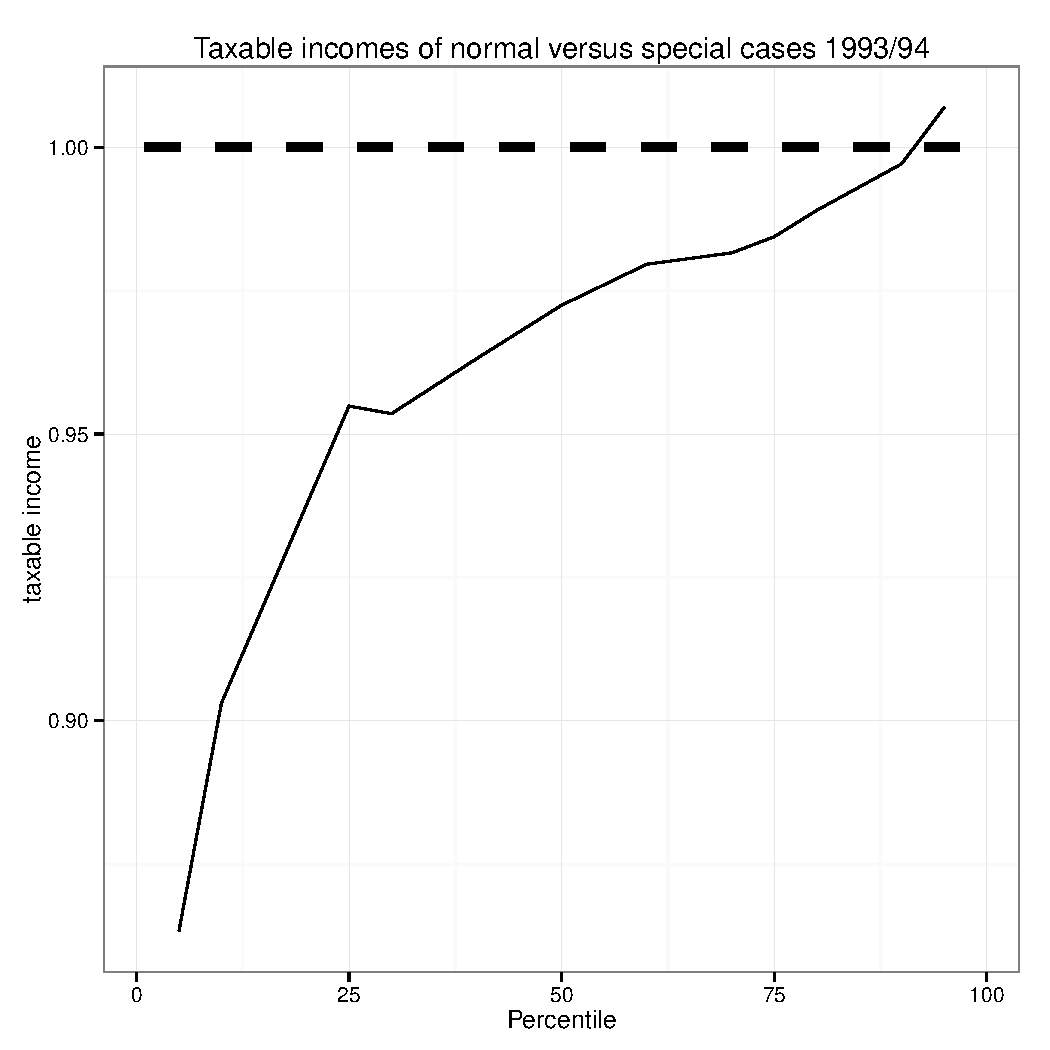
\includegraphics[width=\maxwidth]{figure/specialcases9394} \caption[Comparison of normal and special cases 1993/94]{Comparison of normal and special cases 1993/94\label{fig:specialcases9394}}
\end{figure}


\end{knitrout}

%latex.default(format(c(`Median Index` = med, `Lower Index` = lower,     `Upper Index` = upper, `$\\Delta$ Gini` = dgini), digits = ndig),     file = "", title = title, where = "H", label = tablabel,     caption = caption)%
\begin{table}[H]
\caption{\label{pol9394spec}} 
\begin{center}
\begin{tabular}{ll}
\hline\hline
\multicolumn{1}{l}{Inequality Indices}&\multicolumn{1}{c}{}\tabularnewline
\hline
Median Index&0.020\tabularnewline
Lower Index&0.029\tabularnewline
Upper Index&0.010\tabularnewline
$\Delta$ Gini&0.013\tabularnewline
\hline
\end{tabular}\end{center}

\end{table}


1993/94 a pooled data set of normal and special cases has a slightly higher density at both ends compared to data based in normal cases only (see figure \ref{fig:specialcases9394}). Special cases appear to have a slightly lower median income and their distribution is more skewed. Therefore special cases are more polarized than normal cases (see table \ref{pol9394spec}), i.e. striving away from the median (positive Median Index of 0.02). This tendency is more pronounced in the lower than upper part  of the distribution (Lower Index of 0.029 compared to Upper Index if 0.01). 
As the special cases consist of a broad mix of individuals it remains unclear which factor explains the differences of both distributions. Possible explanations can be immigrants partly concentrating in lower income percentiles, low income artists who belong to the special cases or a more technical selection effect: tax units not liable for taxation throughout the whole year are special cases; those cases might have lower incomes, e.g. if they moved and stopped working. To get a more complete picture we can look how the two distributions relate to each other in 2010 (see figure \ref{fig:specialcases10}).

% Variante 2010


\begin{knitrout}
\definecolor{shadecolor}{rgb}{0.969, 0.969, 0.969}\color{fgcolor}\begin{figure}[H]

\includegraphics[width=\maxwidth]{figure/specialcases10} \caption[Comparison of normal and special cases 2010]{Comparison of normal and special cases 2010\label{fig:specialcases10}}
\end{figure}


\end{knitrout}

%latex.default(format(c(`Median Index` = med, `Lower Index` = lower,     `Upper Index` = upper, `$\\Delta$ Gini` = dgini), digits = ndig),     file = "", title = title, where = "H", label = tablabel,     caption = caption)%
\begin{table}[H]
\caption{\label{pol2010spec}} 
\begin{center}
\begin{tabular}{ll}
\hline\hline
\multicolumn{1}{l}{Inequality Indices}&\multicolumn{1}{c}{}\tabularnewline
\hline
Median Index&0.031\tabularnewline
Lower Index&0.039\tabularnewline
Upper Index&0.022\tabularnewline
$\Delta$ Gini&0.020\tabularnewline
\hline
\end{tabular}\end{center}

\end{table}


2010 the picture is similar but more apparent: Special cases appear more frequent around the lower percentiles of the pooled distribution (Lower Index of 0.039), however 2010 there is a more noteworthy effect in the upper part of the distribution (Upper Index of 0.022). According to figure \ref{fig:specialcases10} we can attribute this effect to the top percentiles. This gives credibility to the thesis that rich immigrants whose number increased between 1994 and 2010 drive the effect.

% Auf neuste Zahlen anpassen

%As we can see from figure~\ref{fig:specialcases93942} and \ref{fig:specialcases092}, special cases differ strongly 
%from normal cases within the low and top percentiles. Within the tax period 1993/94 the fifth percentile of 
%normal cases is 15.8\% higher than the fifth percentile of the combines data while the 95\% percentile of 
%normal cases is even 0.7\% lower if one leaves out special cases. This indicates special cases are very 
%different from normal cases as the share of special cases is only 15.5\%.\footnote{1993/94 there were 2.76 
%million tax units defined as being normal cases compared to 0.51 million special cases.}
%In 2009 the situation has the same pattern. The fifth percentile of normal cases has 11\% higher taxable 
%income compared to data where special cases are included. The five percent top incomes are 4.9\% higher 
%within all cases compared to normal cases only. The share of special cases however decreased 
%to 7.2\%.\footnote{2009: 3.42 million normal cases, 0.27 million special cases}



\emph{taxable income with and without non-taxed}

FTA-Tax statistics sometimes exlcude tax units, which reach below the treshold to be taxed (let's call them zeros). We compare here three Gini-time-series \ref{fig:with_without_zeros_Gini}. Excluding zeros leads to a dramatical drop of the gini-coefficent, which is not realy surprising. On the other hand inequality is overestimated when assuming non-taxed tax units have zero taxable income. Rather we must assume taxable income for zeros lay between zero and the taxation treshold. We adress this by presenting a third time-series, where we assume non-taxed have a taxable income equal halve the threshold for single tax units (around CHF 8000). This results slightly lower Gini-coefficents.

% Beim Vergleich der Datensätze unterschieden nach nur besteuerten und unter berücksichtigung der nicht besteuerten, stellt sich die Frage wie die unteren Einkommen imputiert werden. Wir haben uns überlegt, dass dies vor allem singles (übrige) betrifft, weil Familien in den unteren Einkommenstabellen bereits sehr selten vorkommen. Deswegen reicht es nur die Untergrenze für singels zu berücksichtigen. Diese liegt 2010 bei 16'900 verändert sich aber über die Zeit

\begin{knitrout}
\definecolor{shadecolor}{rgb}{0.969, 0.969, 0.969}\color{fgcolor}\begin{figure}[H]

\includegraphics[width=\maxwidth]{figure/with_without_zeros_Gini} \caption[Gini coefficients with, without and imputed non-taxed units]{Gini coefficients with, without and imputed non-taxed units\label{fig:with_without_zeros_Gini}}
\end{figure}


\end{knitrout}

% Wenn wir annehmen, dass die Brülhart-Daten, sowohl die unteren als auch die oberen Perzentile angemessen abbildend, dann reicht der Vergleich. Etwas merkwürdig ist es jetzt, wenn wir die Gini-Reihe mit den ESTV Daten machen und dann den Vergleich mit den Brülhartdaten

%<<with_without_zeros_RelDist_mitBruelhart,warning=FALSE, fig.cap='',fig.pos='H'>>=
%bd.2010 <- filter(read.csv("../../data/data_Schweiz.csv", header=TRUE,sep=";"),Veranlagungsperiode==2010,Einheit=="Total")
%bd.0.2010 <- filter(read.csv("../../data/data_Schweiz_mitNull.csv", header=TRUE,sep=";"),Veranlagungsperiode==2010,Einheit=="Total")
%start <- which(names(bd.2010)=="p1")
%end <- which(names(bd.2010)=="p99_99")
%percentile <- c(1,5,10,20,25,30,40,50,60,70,75,80,90,95,96,97,98,99,99.5,99.9,99.99)
%bd.2010<- data.frame(t(bd.2010[1,start:end]),percentile)
%names(bd.2010)[1]=c("inc")
%bd.0.2010<- data.frame(t(bd.0.2010[1,start:end]),percentile)
%names(bd.0.2010)[1]=c("inc")

%bd.0.2010 <- rbind(c(0,0),bd.0.2010)
%ival<-bd.0.2010$inc
%perval<-bd.0.2010$percentile
%bd.0.2010.ind<-unlist(sapply(2:length(ival),function(i){
 % len=(perval[i]-perval[i-1])*100
%  seq(ival[i-1],ival[i],length.out=len)
%}))

%bd.2010 <- rbind(c(0,0),bd.2010)
%ival<-bd.2010$inc
%perval<-bd.2010$percentile
%bd.2010.ind<-unlist(sapply(2:length(ival),function(i){
%  len=(perval[i]-perval[i-1])*100
%  seq(ival[i-1],ival[i],length.out=len)
%}))


%par(mfrow=c(1,2))
%# Prop-Density Plot
%density1 <- density(log(bd.2010.ind))
%plot(x = (density1$x), y = density1$y, type = "l",
%     xlab = "taxable income", ylab = "density"
%     #axes = FALSE,
%     #xlim = c(-50, 200),
%     #ylim=c(0,0.0116031)
     )
%title(main="all tax units vs without non-taxed",cex=0.6)
%axis(side = 1)
%axis(side = 2)
%fig1legend <- list(x=c(6,6),y=c(0.6,0.6))
%legend(fig1legend,lty=1:2, bty="n",
%       legend=c("without non-taxed","all tax units"))
%density2 <- density(log(bd.0.2010.ind))
%lines(x = (density2$x), y = density2$y, type = "l",lty=2)


%# Relative Distribution

%gA0 <- reldist(y=bd.2010.ind, yo=bd.0.2010.ind,
%               smooth=0.4, ci=FALSE,
%               show="residual",
%               bar=TRUE, quiet=FALSE,
%               ylim=c(0.5,2), ylab="",
%               discrete=FALSE,
%               xlab="Proportion of 2010 Distribution (including non-taxed)")
%title(main=paste("Effect of different shape"))
%abline(h=1,lty=2)

%par(mfrow=c(1,1))
%@


%<<polindexzeros, results='asis'>>=
%polTable(bd.2010.ind,bd.0.2010.ind,tablabel="polzeros")
%@

% Wenn etwas bei den unteren Perzentilen nicht stimmt (nicht Besteuerte als Null gewertet), dann müsste der Vergleich mit den ESTV-Nullern gemacht werden.
% Es ist mir aktuell unklar bei welchem Datensazt jetzt die Perzentile mit imputierten Nullern vorliegt.

%Including zeros leads to significantly higher gini coefficients. However we must keep in mind, that these might be artificially high values as we assume zero income for everyone in the zero group. We can conclude more from the graphic: the ratio between both measures seems to be quite constant although for aggregate Switzerland but there are minor deviations for multiple cantons as well as strong deviations for the cantons Geneva and Ticino. However the problems seem not to result from a shift in the zero-share over time but they are specific for the time-period when the tax system changed. 

\emph{comparison of tax-data and survey data distribution}




\begin{knitrout}
\definecolor{shadecolor}{rgb}{0.969, 0.969, 0.969}\color{fgcolor}\begin{figure}[H]

\includegraphics[width=\maxwidth]{figure/BruelhartvsHABE} \caption[Comparison of tax and survey data]{Comparison of tax and survey data\label{fig:BruelhartvsHABE}}
\end{figure}


\end{knitrout}


\begin{knitrout}
\definecolor{shadecolor}{rgb}{0.969, 0.969, 0.969}\color{fgcolor}\begin{figure}[H]

\includegraphics[width=\maxwidth]{figure/BruelhartvsHABEmarried} \caption[Comparison of tax and survey data for married]{Comparison of tax and survey data for married\label{fig:BruelhartvsHABEmarried}}
\end{figure}


\end{knitrout}


\begin{knitrout}
\definecolor{shadecolor}{rgb}{0.969, 0.969, 0.969}\color{fgcolor}\begin{figure}[H]

\includegraphics[width=\maxwidth]{figure/BruelhartvsHABEunmarried} \caption[Comparison of tax and survey data for unmarried]{Comparison of tax and survey data for unmarried\label{fig:BruelhartvsHABEunmarried}}
\end{figure}


\end{knitrout}

From the discussion in the data section we would expect differences between the income distributions from survey and tax data. Within the FTA data we observe zeros for incomes below the threshold to be liable for federal tax while survey data might cover this range. On the other hand we expect underreporting from both lowest percentiles and highest percentiles (middle class bias) within the survey data. Figure \ref{fig:BruelhartvsHABE} (left) however reveals a more critical issue related to tax data, that is the median location of income compared to survey data. Although we try to measure similar concepts of income, survey data shows a median (93.000 CHF) more than twice as big as tax data (44.600 CHF). The issue here is clearly the assumptions of household composition. While survey data is likely to capture the correct household composition, tax data can only approximate households by using marital status. Splitting the data in married and unmarried tax units underpins this argument. From figure \ref{fig:BruelhartvsHABEmarried} we can see that married tax units (FTA data) and household with married couples (survey data) are better (but still not perfectly) comparable. Figure \ref{fig:BruelhartvsHABEmarried} (right) shows the expected shape difference between the two distributions:  survey data has a bias towards the (median-adjusted) 80\% to 90\% percentile (of the FTA data distribution). Top percentiles are badly covered by survey data, suggesting that inequality measures based on survey data might underestimate inequality development that arises from changes in the incomes of the rich. Though, survey data can be of interest if one is interested in the lower 20\% of the income distribution. 

The bad household approximation within tax data needs to be addressed in further research. One possible way would be to link tax data to household ID's from the residential register.


\subsection{Intertemporal comparison}



\begin{knitrout}
\definecolor{shadecolor}{rgb}{0.969, 0.969, 0.969}\color{fgcolor}\begin{figure}[H]

\includegraphics[width=\maxwidth]{figure/benplot} \caption[Gini coefficients over time]{Gini coefficients over time\label{fig:benplot}}
\end{figure}


\end{knitrout}

Figure\ref{fig:benplot} displays the most relevant Gini-coefficients that can be calculated for Switzerland. Although we can not adjust the Gini-coefficients to be perfectly valid, we can discuss the picture against the background of our analyses. For the periods before the second world war it is difficult to draw secure conclusions because these data points are based on unreliable data. 1933 only 13.7\% of the population filled in a tax form \citep{dell_income_2005}. During the war we see a tendency towards lower income inequality. This might be attributable to a changed data base as the amount of non-fillers decreased during the war and shortly after. The period after the world war is characterized by strong economic growth as well as an increase in inequality. Our interpretation is that high income percentiles disproportionately profited from the economic upturn. After the oil crises there were alternating phases of social welfare expansion and economic upturns.

The more interesting part of the picture are the years around and past the millennium. Between 1997/98 and 2003 we see a gap in the FTA series caused by the change in the tax system. Our approach to impute the gap is to interpolate the income sums of all FTA-reported income brackets. This is fruitful because cantons switched the tax system in different years so we gain at least some information about the trend within the gap. The spike 2001 can be explained by tax tricks: within the period the tax system changed, individuals were able to save taxes by shifting parts of their incomes into this period. 

After the financial crisis most of the data sources (except EU SILC) state decreasing inequality. Our interpretation is that top percentiles lost relevant parts of their incomes from capital investments. 

%%%-------------------------------------------------%%%
%%% Include discussion %%%
%%%-------------------------------------------------%%%


%%%-------------------------------------------------%%%
%%% Sub document for discussion %%%
%%%-------------------------------------------------%%%

\section{Discussion}

This article highlights the main disparities between taxdata based assessment of inequality opossed to given standard concepts of inequality as it is mainly applied with household-surveys. We reflected all important concerns based on the case of Switzerland. Can we measure what we want to measure? Do data include the cases we are interested in? The paper revealed tax data afflicted with numerous problems when it comes to analyzing inequality. On the pro side tax data is not a sample but covers the full population liable to federal tax. The documentation of tax data for almost 100 years makes it the only option if the researcher is interested in long term analyses of swiss income inequality, take it or leave it. On the contra side the researcher needs to keep in mind several limitations. According to our analyses we can give advice which issues are more or less serious. The biggest issue is that tax data does not capture households. In comparison to survey data we have seen that tax data extremely overestimates the share of singles/single households if we assume marital status to be a proxy for household composition. Luckily there is a way to fix this shortcoming for further research. For analyses of household income inequality, the researcher should gather household information, e.g. by linking tax data to the population register. The second most important drawback of tax data is the non-reporting of the non-taxed (low income) tax units. The best solution here would be to gather data directly from the FTA where these information are available, although not published. As a minimum the researcher should keep an eye on the share of population ``disappearing'' below the threshold. The larger the share, the more likely it is to overlook increases in inequality if tax data is used without these cases. 
Minor issues are whether the researcher looks at all cases (including special cases) the FTA may provide or only normal cases. However this issue became more relevant in recent years as high income special cases became more frequent. Our recommendation is to use both normal and special cases wherever possible but it is not an important issue. It is also not very important for the researcher whether the researcher looks at equivalized or non-equivalized incomes as long as the exact household structure is unknown. A more fruitful approach is to do separate analyses for married and unmarried tax units and treat the latter with healthy portion of caution.

% Hier könnte allenfalls der Bogen zur Theorie gespannt werden 

%Methodological Main findings 
%(1) Tax data is useful because it's possible to construct consistent measures over time for income and wealth, which is useful to asses changes over time and conducted studies about impact of structural changes.(2) Concerning accuracy of inequality tax data has advantages and shortcomings. It's superior to survey data, because the latter is affected by non-responded bias. Tax data includes data about the whole population [was finden wir wegen den Nullern raus] . or at least it should (tax evasion).(3) The FTA-Tax data has different shortcomings, which cannot be handled like a measure of income and wealth which (a) cannot be corrected for household size and (b) is neither a pre-transfer nor a post-transfer income measure. Therefor it's comparability with other surveys is harsh as long as the main sources of data on inequality are based on measures, which cannot be replicated with taxable income. This FTA-Tax data problem can be handled with non-aggregated tax-data .


%Main findings for Switzerland (1) Our data suggests that income inequality overall slightly increased in Switzerland and we might distinguish three episodes: 1. Substantial increase in times of economic growth 1950 to 1974 ending with the oil crisis 2. Ups and downs from 1970 to 2000 3. Relatively steep increase in inequality in the early 2000s
%(2) Despite the recent increase, overall income inequality in Switzerland is not very high in international comparison. With respect to inequality in wealth, however, Switzerland takes a leading position in the world.
%(3) While the overall Swiss inequality remained pretty stable over decades, inequality between cantons underwent a bizarre development.

% Mögliche Einstiegsfloskel
% This article highlights the main disparities between taxdata based assessment of inequality opossed to given standard concepts of inequality as it is mainly applied with household-surveys. We reflected all important concerns based on the case of Switzerland.

%%%-------------------------------------------------%%%
%%% Include acknowledgements %%%
%%%-------------------------------------------------%%%


%%%-------------------------------------------------%%%
%%% Sub document for acknowledgement %%%
%%%-------------------------------------------------%%%

\section{Acknowledgements}

We thank Ben Jann, Robert Fluder and Tobias Fritschi for helpful comments on the article. We also like to thank Stefan Ilic for the prepartion of the data set.

%%%-------------------------------------------------%%%
%%% Include the bibliography %%%
%%%-------------------------------------------------%%%


\end{multicols}

\bibliography{bibliography/bib} 

%%%-------------------------------------------------%%%
%%% Include the appendix %%%
%%%-------------------------------------------------%%%


%%%-------------------------------------------------%%%
%%% Sub document for appendix %%%
%%%-------------------------------------------------%%%

\section{Appendix}



\end{document}
